\documentclass[11pt]{article}

\usepackage[T1]{fontenc}
\usepackage[utf8]{inputenc}
\usepackage{lmodern}
\usepackage[margin=1in]{geometry}
\usepackage{microtype}
\usepackage{placeins}
\usepackage{seqsplit}
\setlength{\emergencystretch}{2em}
\newcommand{\sig}[1]{\texttt{\seqsplit{#1}}}
\usepackage{amsmath}
\usepackage{amssymb}
\usepackage{booktabs}
\usepackage{longtable}
\usepackage{tabularx}
\usepackage{array}
\usepackage{multirow}
\usepackage{enumitem}
\usepackage{xcolor}
\usepackage{graphicx}
\usepackage{tikz}
\usetikzlibrary{arrows.meta,positioning,shapes.geometric,fit,backgrounds,calc}
\usepackage{algorithm}
\usepackage{algpseudocode}
\usepackage{listings}
\usepackage[numbers,sort&compress]{natbib}
\usepackage[colorlinks=true,linkcolor=blue!55!black,citecolor=blue!55!black,urlcolor=blue!55!black]{hyperref}
\usepackage[nameinlink,noabbrev]{cleveref}
\crefname{lstlisting}{listing}{listings}
\crefname{algorithm}{algorithm}{algorithms}

\lstdefinestyle{json}{
  basicstyle=\ttfamily\footnotesize,
  frame=single,
  rulecolor=\color{black!30},
  backgroundcolor=\color{black!2},
  breaklines=true,
  columns=fullflexible,
  keepspaces=true
}
\lstdefinestyle{js}{
  basicstyle=\ttfamily\footnotesize,
  frame=single,
  rulecolor=\color{black!30},
  backgroundcolor=\color{black!2},
  breaklines=true,
  columns=fullflexible,
  keepspaces=true,
  language=JavaScript
}

\newcommand{\system}{\textsc{OPAL}}
\newcommand{\ah}{\textsc{Academic Harness}}
\newcommand{\dsh}{\textsc{DeepSeek Harness}}

\hypersetup{
  pdftitle={OPAL: Oracle-Preserving Autonomous Lessons for Local Academic Harness Adaptation},
  pdfauthor={Raktim Mondol},
  pdfkeywords={oracle-preserving, autonomous lessons, local self-improvement, academic harness, evaluation}
}

\title{OPAL: Oracle-Preserving Autonomous Lessons for Local Academic Harness Adaptation}
\author{Raktim Mondol\\Academic Harness Project}
\date{October 2026}

\begin{document}

\maketitle

\begin{abstract}
Research agents increasingly operate inside long-lived harnesses that supply tools, memory, context construction, and execution policy. A fixed harness forces users to restate conventions, while autonomous harness rewriting risks changing the checks that establish scientific integrity. We present \system{} (Oracle-Preserving Autonomous Lessons), a local lesson-learning layer for an academic research harness built as a plugin for \dsh{}. The layer captures tool outcomes, audit findings, gate decisions, user corrections, and explicit preferences; diagnoses recurring failures across eleven research task classes; admits short lessons automatically; injects them into later turns; and compares injected against eligible control turns to promote, quarantine, or retire lessons. Its mutable surface is lesson text only. The deterministic audit engine, plugin code, project files, and evaluation logic remain outside the loop, following the fixed-evaluator principle. The store is local by default; an optional remote judge is veto-only and receives lesson text and evidence counts, never manuscript text. We report 96 automated RSI checks, 17 passing plugin test suites, and a nine-document corpus experiment. On 690 units and 584 citations, the audit produced 1,158 findings; 31/31 injected defects were detected, and leave-one-project-out lessons covered 23/23 specific finding families at about four times the token cost of a generic lesson. Held-out routing and safety tests exposed limits: 56.7\% accuracy on a hand-labeled routing set and 0.53 F1 on paraphrased unsafe lessons. We assess the system against the survey's Selection, Activation, Attribution, and Improvement criteria and identify the controlled studies needed before claiming causal research-quality gains.

\end{abstract}

\section{Introduction}
\label{sec:intro}

Research work is cumulative but rarely repetitive in the same way. A researcher who writes one manuscript and then another expects the assistant to remember how their evidence is registered, how numbers are bound to data, which statistical checks matter, what a funder requires, and how they prefer to revise. A static agent harness does not accumulate that experience. The user either repeats instructions or edits the harness by hand. The alternative, letting the agent rewrite its own harness, is attractive but dangerous: the harness includes the checks that decide whether a citation exists, whether a number matches its source, and whether a claim is supported.

Harness self-evolution studies this trade-off under a fixed base model. A harness $H$ supplies tools, context construction, memory, and execution control; a run produces trajectories scored by an evaluator $J$; and an update rule revises the persistent harness state for later runs \citep{wei2026harnessrsi,wei2026selfevolvingagentharness}. The survey distinguishes \emph{interpreted} updates, which revise instructions, memory, or coordination specifications read by fixed components, from \emph{executable} updates, which revise tools, repository logic, or plugin composition. It also separates self-evolution, the update process, from self-improvement, a beneficial change established through evaluation. The distinction matters because an update can persist without improving anything.

The empirical picture is sobering. Across 93 primary reported comparisons in the survey, none satisfy all four evaluation criteria---Selection, Activation, Attribution, and Improvement---and only seven satisfy three. Full evidence for Activation appears in 8 comparisons and for Attribution in 10; most reports establish only that an artifact was available, not that it executed in the scored runs or that its effect survived matched compute and execution variance \citep{wei2026harnessrsi}. At the same time, self-improving systems can fail in ways that are especially costly in science: they can modify verification logic rather than the behavior under test \citep{wang2026tampering}, write checks that do not correspond to observed failures \citep{wang2026phantom}, rely on self-authored verification \citep{guo2026selfverification}, inflate reward through stored memory \citep{asadolahi2026inflation}, or overfit a reusable holdout \citep{dwork2015reusable,cawley2010overfitting}. Model--harness interactions add another confound: a gain attributed to the harness may depend on the model, the scaffold, or the evaluation protocol \citep{li2026rightfit,tian2026ceiling}.

This paper takes the conservative branch of that evidence. We describe \system{}, an oracle-preserving local lesson-learning layer integrated into \ah{}, a research plugin for \dsh{} \citep{academicharness2026,deepseek2026harness}. \ah{} supplies scientific search, dataset and policy lookup, citation and integrity checks, statistical and figure audits, a paper-memory layer \citep{papermemory2026}, and a deterministic writing oracle built around a vendored \texttt{ah} engine. The engine inventories units, numbers, citations, facts, and claims; records findings in a ledger; and closes a gate only when the current turn introduced no open blocker or major. The plugin also exposes an author-only approval path for waivers, fact proposals, plans, and disclosures. These properties make the plugin a useful testbed: there is already a fixed evaluator, a persistent project state, and a clear distinction between what the agent may read and what it may change.

\system{} adds a learning loop around that substrate. It captures structured outcomes from every research turn, diagnoses recurring failures, admits short textual lessons from a remedy catalogue, injects them into later turns, and uses a trial/control comparison to promote, quarantine, or retire them. Three design choices follow directly from the survey. First, the loop only edits interpreted state. It never rewrites the plugin, the vendored engine, the project, protected paths, or the audit logic. Second, the evaluator stays outside the candidate's editable surface. Third, learning is local and reversible: the store is on the user's machine, every lesson is visible and forgettable, and an optional remote judge can veto but not admit.

The contributions are:
\begin{itemize}[leftmargin=1.4em,itemsep=2pt]
  \item A design for evaluator-preserving local RSI in an academic research agent, including requirements, mutable/immutable boundaries, task scoping, and a lesson lifecycle.
  \item A concrete implementation in a production plugin: capture hooks, a local append-only store, an eleven-class research task taxonomy, a remedy catalogue, safety lints, an in-session tool, an offline CLI, and three benchmarks.
  \item Safety and privacy mechanisms suited to research work: a local judge, a veto-only remote option, negation-aware lesson filtering, symlink-safe defect injection, immutable-oracle checks, and fail-soft integration with the writing loop.
  \item A nine-document corpus experiment on three manuscripts and six proposals: 31/31 injected defects detected, 23/23 specific finding families covered by leave-one-project-out lessons, about 3.9$\times$ the token cost of a generic lesson, and negative results on task routing and held-out safety paraphrases.
  \item A preliminary validation and an explicit self-assessment against the survey's four evaluation criteria. We report what the tests establish and what they do not: the implementation is exercised on real documents, but no controlled model or user study yet shows that the lessons improve research quality.
\end{itemize}

We do not train model weights, generate executable tools at runtime, or claim that a lesson is evidence. The system is a learning layer for a research harness, not a replacement for the researcher's judgment or the audit engine's checks.

\section{Related Work}
\label{sec:related}

\subsection{Harness self-evolution}
A harness is the software and configuration that governs how a base model operates in an environment. The survey by \citet{wei2026harnessrsi} formalizes a run as $\tau \sim \mathrm{Run}(M,H,E)$ scored by an evaluator $J$, and an update as $H_{k+1}=\mathrm{Update}(H_k,\mathcal{B}_k)$ over a batch of trajectories. The evaluator remains outside the candidate's editable surface; internal critics and provisional verifiers may belong to the mutable harness, but they do not define admission. The survey organizes update targets into interpreted state (prompts, memory, reusable procedures, workflows) and executable state (tools, code patches, repository logic, plugin composition), and separates the update mechanism from the evidence that an update helped. Our work adopts the interpreted side of this taxonomy and the fixed-evaluator boundary, but specializes both to a local academic research harness.

\subsection{Experience mining and procedural memory}
Reflexion stores verbal reflections on failures and reloads them for another attempt \citep{shinn2023reflexion}. ExpeL extracts cross-task insights from a pool of trajectories and curates them with add, edit, and vote operations \citep{zhao2024expel}. AWM induces recurring sub-goal workflows from trajectories \citep{wang2025workflow}; Agent KB maintains a cross-domain experience base whose top-$k$ items are injected into later runs \citep{tang2025agentkb}; ReasoningBank consolidates reasoning strategies from successes and failures into a bank injected into the system instruction \citep{ouyang2026reasoningbank}. MemP compares procedural-memory update strategies and abstraction granularities \citep{fang2026memp}. Trace2Skill distills execution lessons into skill patches \citep{ni2026trace2skill}; SkillClaw admits a candidate skill only if it beats the deployed pool on validation tasks \citep{ma2026skillclaw}; GSE learns globally reusable skills under project-held-out splits \citep{yang2026gse}; and GSkill learns \texttt{SKILL.md} files for coding agents from prior runs \citep{tan2026gskill}.

\system{} resembles this line in its unit of learning (short textual lessons) but differs in three ways. It learns from a stream of real research turns rather than an offline training pool; it scopes lessons by a deterministic research-task taxonomy; and it is built around an existing deterministic writing oracle rather than a benchmark harness. The store is deliberately small: a lesson is a sentence or two, not a workflow graph.

\subsection{Gated consolidation and skill libraries}
ACE grows and consolidates an evolving context playbook through incremental delta updates \citep{zhang2026agentic}; Dynamic Cheatsheet maintains an adaptive memo of strategies at test time \citep{suzgun2026dynamic}; SkillOpt evaluates a revised skill set on validation before replacing the active library \citep{yang2026skillopt}; SkillOpt-Lite adds a validation deadband plus compilation and smoke tests \citep{shen2026skilloptlite}; and VALVE admits revisions through paired comparisons on a validation panel \citep{wang2026valve}. At the library level, Ratchet asks how reliable a judge must be before a skill may be retired \citep{zhang2026ratchet}; SkillsVote governs a skill lifecycle through collection, recommendation, and voting \citep{liu2026skillsvote}; Library Drift diagnoses silent drift in a growing self-evolving library \citep{zhang2026librarydrift}; and pre-commit gating checks proposed skill changes before commit \citep{shang2026backfires}.

Our lesson lifecycle borrows the trial/admit/retire structure but not the offline validation panel. New diagnosis lessons begin as trials with a randomized holdout; active lessons retain a small ongoing control sample; a lesson that loses to control is quarantined; and a lesson that never beats control is retired. Explicit user preferences are active immediately but remain subject to a time-to-live and can be forgotten. The design is closer to a lightweight online bandit than to a centralized skill library, because the target is one user's local research workflow.

\subsection{Prompt and workflow optimization}
APE proposes instructions and keeps the highest-scoring candidate \citep{zhou2023large}; OPRO feeds earlier instructions and scores to an optimizer model \citep{yang2024large}; TextGrad backpropagates textual critiques through a graph of model calls \citep{yuksekgonul2025textgrad}; GEPA uses execution-trace reflection and Pareto selection \citep{agrawal2026gepa}; DSPy compiles declarative pipelines while control flow stays fixed \citep{khattab2024dspy}; and AFlow searches workflows expressed as operator-composing code \citep{zhang2025aflow}. These methods generally assume a dataset, a scalar metric, and an offline optimization budget. \system{} has none of the three in a stable form: the task stream is non-stationary, the outcome is a heuristic composite of tool signals, and the budget is the user's own session. We therefore use a deterministic remedy catalogue and online trial/control evidence rather than gradient-like prompt search.

\subsection{Executable and repository-level self-improvement}
SICA lets the best archived agent revise its own multi-file Python codebase \citep{robeyns2025selfimproving}; DGM branches repository variants into an open-ended archive \citep{zhang2026darwin}; HGM allocates lineage-expansion and evaluation budgets by Thompson sampling \citep{wang2025huxley}; DarwinX evolves repository-level candidates through selection, mutation, and recombination \citep{zhang2026darwinx}; MOSS rewrites routing, hooks, state management, and dispatch code and swaps the container behind a health check plus human authorization \citep{cai2026moss}; Ouroboros evolves its core through reviewed commits \citep{razzhigaev2026ouroboros}; and AgentDevel uses versioned diffs and release-candidate regression tests \citep{zhang2026agentdevel}. Self-Harness, HarnessCompass, HarnessFix, HarnessX, and HarnessBank edit declared harness components, optimize components separately, diagnose failures, bind updates to hooks, or archive patches under an immutable evaluation kernel \citep{zhang2026selfharness,zhang2026harnesscompass,chen2026harnessfix,chen2026harnessx,luo2026harnessbank}. Harness Ceiling compares harness edits on long-horizon planning to identify failures that remain for weight training \citep{tian2026ceiling}.

We deliberately exclude this class from the runtime loop. The survey reports weak Activation and Attribution for executable patches, and the academic failure modes are asymmetric: a code patch that weakens a check can make every later manuscript look compliant. In \system{}, executable changes require normal plugin development, review, and release. The loop's autonomy is limited to lesson text.

\subsection{Evaluation and failure modes}
The survey grades each primary comparison on four claims. \emph{Selection} asks whether reporting outcomes were separated from proposal, ranking, admission, and report choice. \emph{Activation} asks whether the accepted update operated in the scored runs, with available, reached, and carried as distinct levels. \emph{Attribution} asks whether the update was isolated, inference resources were controlled, and the margin exceeded measured execution variation. \emph{Improvement} asks about task distance between the update and the reported evaluation. The survey's evidence shows the field is strongest on held-out task distance and weakest on Activation and Attribution \citep{wei2026harnessrsi}.

Specific failure modes motivate our safeguards. SWE-bench+ documents solution leakage and weak assertions that corrupt promotion and reporting \citep{aleithan2024swebenchplus}. Phantom Guardrails describes harnesses that fix failures which never occurred \citep{wang2026phantom}. Harness Tampering examines candidates that modify verification logic rather than the behavior under test \citep{wang2026tampering}. Self-Authored Verification finds self-written checks unreliable as admission evidence \citep{guo2026selfverification}. Memory Reward Inflation shows that stored memory can inflate reported reward rather than improve behavior \citep{asadolahi2026inflation}. Spontaneous reward hacking appears in iterative self-refinement \citep{pan2024spontaneous}. Model--Harness Fit and Harness Ceiling warn that gains may not transfer across model--harness pairs or may be bounded by weight-level limitations \citep{li2026rightfit,tian2026ceiling}. Agents That Matter argues that agent comparisons confound capability with cost \citep{kapoor2025matter}.

The statistical tools are equally relevant. The survey derives a confidence-gated admission rule from Hoeffding bounds \citep{hoeffding1963probability}; the reusable-holdout literature explains why repeated adaptive use of one holdout invalidates naive inference \citep{dwork2015reusable}; selection overfitting describes the bias introduced by choosing the best of many evaluated candidates \citep{cawley2010overfitting}; the Ladder mechanism stays reliable under repeated adaptive submissions \citep{blum2015ladder}; and stability-based generalization bounds connect sensitivity to individual observations with the generalization gap \citep{shalev2010learnability,hardt2016train}. \system{} does not claim to satisfy the survey's formal gate. It records the ingredients---proposal data, admission evidence, injected/control outcomes, and a reporting ledger---that a later controlled study would need.

\subsection{Academic research harnesses}
\dsh{} is a plugin-based agent runtime with declared dependencies, checkpointing, and replay; the survey notes that its product page reports no empirical self-evolution evaluation \citep{deepseek2026harness,wei2026harnessrsi}. DSH Everything shows that a plugin can generate and retain tools during execution \citep{shen2026dsheverything}. \ah{} is a research plugin for DSH with scientific search, claim memory, citation and integrity checks, statistical and figure audits, and a vendored writing engine \citep{academicharness2026}. The engine is the plugin's substitute oracle: it inventories every number, citation, unit, and declared claim, records findings in a ledger, and gates a turn on blockers introduced by that turn's edits. PaperMemory supplies local, project-scoped, verbatim-anchored paper and claim memory \citep{papermemory2026}. These components make the plugin a natural place for interpreted self-evolution: the oracle already exists, the persistent project state already exists, and the author-only approval boundary already exists.

\system{} differs from prior harness optimizers in its domain, its editable surface, and its evidence posture. It is not a new prompt optimizer, a skill marketplace, or a code-rewriting agent. It is a local sidecar that learns short, scoped lessons for an academic workflow, keeps the deterministic oracle and all executable state fixed, and reports its own evidence against the survey's criteria.

\section{System Context}
\label{sec:context}

\subsection{The Academic Harness plugin}
\ah{} runs as a preset on \dsh{} \citep{academicharness2026,deepseek2026harness}. The preset supplies general research tools (literature and web search, academic database lookup, dataset and policy records, clinical and regulatory records), scientific file inspection, remote compute, a lab notebook, structured scientific results, and specialist subagents. It also mounts a paper-memory layer for papers, claims, and citations \citep{papermemory2026}, a systematic-review ledger, and integrity, citation, statistical, figure, and reproducibility audits. The tool surface is broad by design; the plugin's system prompt routes tasks to the appropriate tool or skill rather than relying on one general-purpose search loop.

When a workspace contains an \texttt{ah.yaml} file, the plugin also activates the \ah{} writing engine. The engine is vendored inside the plugin and is not installed into the host. It parses the \LaTeX{} tree into units, inventories numbers, citations, facts, claims, and anchors, and runs a tiered audit: structure, numeric and fact consistency, bibliography and source registry, claim bindings, coherence, style, and authoring checks. Findings are recorded in a ledger with stable fingerprints and states (open, fixed, waived, decision-needed). A gate closes only when the current turn introduced no open blocker or major. The engine also exposes snapshots, word-level diffs, claim sidecars, provenance records, review items, and author-only decisions such as waiving a finding or approving a plan.

Two properties of this design matter for self-improvement. First, the oracle is deterministic and inspectable. The same context produces the same findings; the engine has a determinism self-check and a report hash. Second, the oracle is already separated from the agent's authority. The agent can request a decision but cannot waive a finding, accept a fact, verify a claim, or approve a disclosure. The author remains the final authority for consequential writing decisions.

\subsection{Mutable and immutable boundaries}
\label{sec:boundaries}
\system{} treats the following as immutable:
\begin{itemize}[leftmargin=1.4em,itemsep=2pt]
  \item plugin source, hooks, tool registrations, and the system prompt;
  \item the vendored \texttt{ah} engine, its checks, ledger, and report hashing;
  \item project files, protected paths, snapshots, facts, sources, and claim records;
  \item the RSI evaluator, admission policy, benchmark manifests, and lint rules.
\end{itemize}
The only mutable state is a local store of short lesson texts and their statistics. This is a deliberate application of the fixed-evaluator principle: the candidate cannot edit the thing that grades it. It also keeps the plugin's release boundary intact. A lesson can be admitted between sessions; a code change cannot.

The store lives under \texttt{\$DSH\_HOME/ah-rsi} by default and can be overridden with \texttt{AH\_RSI\_STORE}. It contains JSONL event and episode logs, append-only lesson snapshots, admission and retirement decisions, and benchmark records. It never contains the manuscript, the full user message, the paper ledger, or credentials. Events keep hashes, counts, tool names, structured signals, and task-class tags. Explicit preferences are stored as the short sentence the user asked to remember.

\subsection{Why research tasks are different}
Academic work differs from coding benchmarks in ways that constrain the learning loop. First, there is no compiler for a research argument. A deterministic audit can catch a missing citation or a number that does not match its fact, but it cannot decide whether the argument is original or whether the evidence supports the claim. The survey makes a similar point: internal critics and provisional verifiers may be useful, but they are not the final evaluator \citep{wei2026harnessrsi}. Second, errors have asymmetric costs. A fabricated citation, a retracted source presented as current evidence, or a statistic reported without its test and sample size can survive a fluent draft and damage a paper, a grant, or a review. Third, research data and manuscripts are often confidential; sending a full trajectory to a remote optimizer is not an acceptable default. Fourth, a researcher's workflow is personal and long-lived: naming conventions, statistical defaults, venues, funders, and review styles vary across projects and change over time.

These constraints point away from offline prompt search and repository-level self-editing, and toward a small, local, reversible layer that learns from the user's own work. The layer should be autonomous enough to avoid a manual approval for every lesson, but bounded enough that a bad lesson cannot change the audit or the project. It should also be legible: the user must be able to see what was learned, why it was learned, and how to remove it.

\subsection{The gap}
The plugin already has feedback (audit findings, gate decisions, review items) and persistent state (ledger, snapshots, claim sidecars, paper memory), but it has no update mechanism that turns that feedback into a persistent harness change. The model does not automatically remember that the user always wants a DOI resolved before citing, that a particular project's numbers live in a fact macro, or that a class of statistics tasks repeatedly needs a pre-report audit. \system{} fills that gap with the smallest update that can persist across sessions and remain auditable: a scoped textual lesson.

\section{Design}
\label{sec:design}

\subsection{Requirements}
\label{sec:requirements}
The design targets eight requirements:
\begin{enumerate}[leftmargin=1.5em,itemsep=2pt]
  \item \textbf{Autonomy.} The loop must admit, inject, promote, and retire lessons without author approval. A manual gate for every lesson would make the feature unusable in daily work.
  \item \textbf{Local first.} Capture and judging must run on the user's machine. Remote evaluation is optional, explicit, and limited.
  \item \textbf{Evaluator preservation.} The audit engine, plugin code, project files, and admission policy must remain outside the candidate's editable surface.
  \item \textbf{Reversibility.} Every learned change must be visible, bounded, and removable. A bad lesson must not require a code release to undo.
  \item \textbf{Task relevance.} Lessons must be scoped to the kind of research work that produced them, not injected indiscriminately.
  \item \textbf{Sidecar behavior.} The learning loop must be fail-soft and must never block the writing, analysis, or review loop.
  \item \textbf{Auditability.} Every admission and retirement must have a reason, evidence counts, and a timestamp.
  \item \textbf{Academic safety.} Lessons must not encourage fabrication, citation invention, verification skipping, data exfiltration, or overclaiming.
\end{enumerate}

\subsection{Overview}
\label{sec:overview}
\Cref{fig:architecture} shows the loop. A research session produces accepted user prompts, tool outcomes, and gate decisions. Capture hooks normalize these into structured events and close them into episodes. The local store holds events, episodes, lesson snapshots, and decisions. Diagnosis clusters recurring signals and maps them to remedy templates. Validation applies lint rules, contradiction checks, evidence thresholds, and an optional veto-only remote judge. Admission assigns a lifecycle state. The injection selector ranks matching lessons and adds a bounded block to a later turn. The outcome monitor updates injected and control statistics; the admission policy promotes, quarantines, or retires lessons.

The immutable plane is drawn separately on purpose. The loop reads audit findings, gate decisions, and tool errors, but it cannot edit the audit, the project, the plugin, or the admission rule. This is the central architectural commitment: the candidate may change what the agent reads, not what judges the agent.

\begin{figure}[t]
\centering
\resizebox{\linewidth}{!}{%
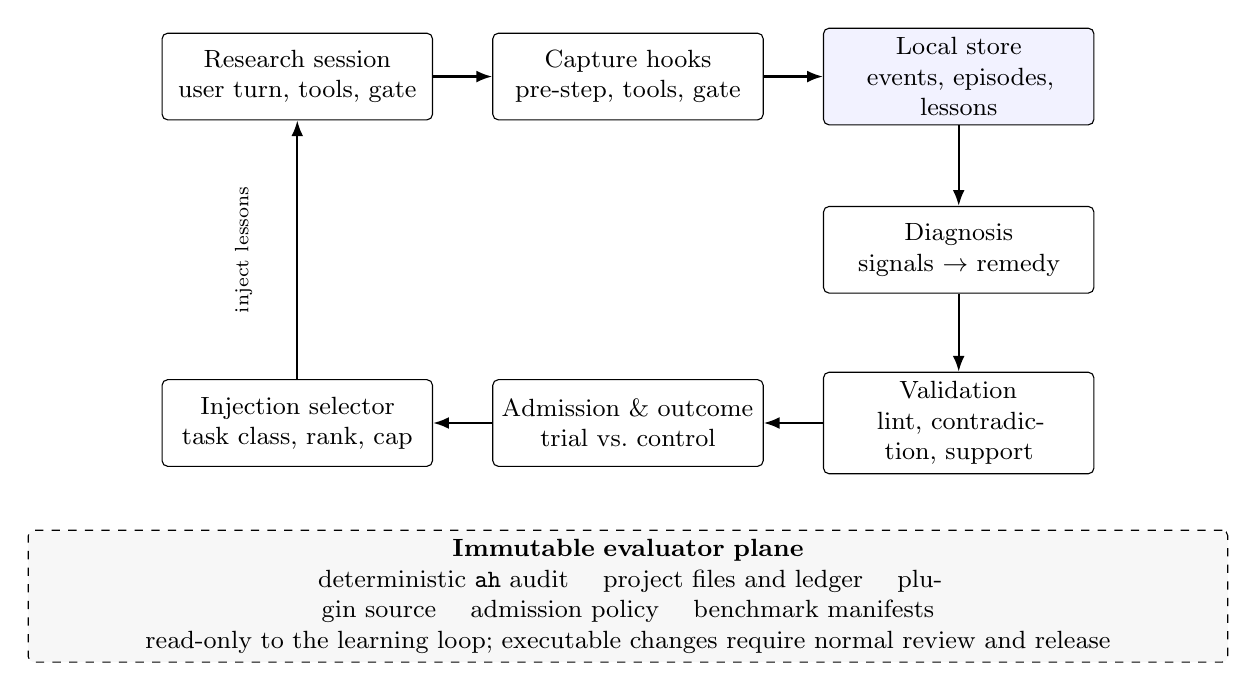
\begin{tikzpicture}[
  font=\small,
  box/.style={draw, rounded corners=2pt, align=center, minimum height=11mm, text width=32mm, fill=white},
  store/.style={box, fill=blue!5},
  immutable/.style={draw, dashed, rounded corners=2pt, align=center, fill=black!3, text width=150mm, minimum height=14mm},
  arrow/.style={-{Latex[length=2mm]}, thick}
]
  \node[box] (session) at (0,0) {Research session\\user turn, tools, gate};
  \node[box] (capture) at (4.2,0) {Capture hooks\\pre-step, tools, gate};
  \node[store] (store) at (8.4,0) {Local store\\events, episodes, lessons};
  \node[box] (diagnose) at (8.4,-2.2) {Diagnosis\\signals $\rightarrow$ remedy};
  \node[box] (validate) at (8.4,-4.4) {Validation\\lint, contradiction, support};
  \node[box] (admit) at (4.2,-4.4) {Admission \& outcome\\trial vs.\ control};
  \node[box] (inject) at (0,-4.4) {Injection selector\\task class, rank, cap};

  \draw[arrow] (session) -- (capture);
  \draw[arrow] (capture) -- (store);
  \draw[arrow] (store) -- (diagnose);
  \draw[arrow] (diagnose) -- (validate);
  \draw[arrow] (validate) -- (admit);
  \draw[arrow] (admit) -- (inject);
  \draw[arrow] (inject) -- (session);
  \node[font=\scriptsize, rotate=90, anchor=south] at (-0.45,-2.2) {inject lessons};

  \node[immutable] (fixed) at (4.2,-6.6) {\textbf{Immutable evaluator plane}\\deterministic \texttt{ah} audit \quad project files and ledger \quad plugin source \quad admission policy \quad benchmark manifests\\read-only to the learning loop; executable changes require normal review and release};
\end{tikzpicture}}
\caption{Architecture of \system{}. The loop is clockwise: capture, store, diagnose, validate, admit, inject. Interpreted lesson state is the only mutable surface. The deterministic audit engine, project state, plugin code, admission policy, and benchmark manifests sit in the immutable plane.}
\label{fig:architecture}
\end{figure}


\subsection{Plugin-layer mapping}
\label{sec:layers}
The general blueprint for RSI in a harness plugin has seven layers: capture, experience store, diagnosis and proposal, frozen evaluator, admission, activation, and observability, tied together by a small operational contract. The implemented architecture covers those layers for lesson-level interpreted state, but it does not implement every possible target. \Cref{tab:layers} states the mapping explicitly.

\begin{table}[t]
\centering
\scriptsize
\caption{Mapping of the general harness-plugin RSI blueprint to the implemented system. The architecture implements the core layers for lesson-level interpreted state. It deliberately does not implement versioned skills, global promotion, or executable changes.}
\label{tab:layers}
\begin{tabularx}{\linewidth}{@{}l>{\raggedright\arraybackslash}p{0.28\linewidth}>{\raggedright\arraybackslash}X@{}}
\toprule
Layer & Implementation & Status \\
\midrule
Capture & Host hooks, gate bus, structured tool and outcome summaries & Implemented. Raw manuscripts and full tool outputs are not stored. \\
Experience store & Append-only JSONL, lesson snapshots, decisions, oracle manifest, risk metadata & Implemented. No database server; local lock. \\
Diagnosis and proposal & Signal clustering, remedy catalogue, task-workflow fallbacks & Implemented as a rule-based proposer. A learned proposer is deferred. \\
Frozen evaluator & Deterministic \ah{} audit, synthetic and corpus benchmarks, oracle manifest & Implemented for deterministic checks. A formal held-out production gate is deferred. \\
Admission & Trial/control, promotion, quarantine, retirement, caps, TTL, explicit rollback & Implemented with a heuristic margin. No formal PAC guarantee; no author approval by design. \\
Activation & Task-class lesson injection, token budget, precedence, reached proxy & Implemented for lessons. Versioned skills and a semantic adherence metric are deferred. \\
Observability & Status, report, cost, reached counts, risk tiers, decisions, export, purge & Implemented. A drift dashboard and encryption at rest are deferred. \\
Contract & Hooks, \texttt{ah\_rsi} tool, CLI, \texttt{rollback} & Implemented. \texttt{diagnose} collapses propose, evaluate, and admit; manual capture is not exposed. \\
Risk tiers & T0 observe; T1 local lessons; T2 local skills/policies; T3 global prompt/skill; T4 executable code & T0--T1 implemented and autonomous; T2 deferred; T3--T4 out of scope. \\
\bottomrule
\end{tabularx}
\end{table}


The main omissions are deliberate. There is no versioned skill-file generator; the lesson is the persistent artifact. There is no global promotion path; the store is local to one user and scoped by task class. There is no runtime code editing; executable changes remain in the normal release process. Within the implemented lesson tier, the system is autonomous: it admits, injects, promotes, quarantines, retires, and rolls back without author approval. The evaluator, project state, plugin code, and admission policy remain fixed.

We use five risk tiers. \emph{T0 observe} captures without injecting. \emph{T1 local lessons} is the implemented tier: short interpreted advice, trial/control admission, caps, TTL, and rollback. \emph{T2 local skills or policies} would add versioned artifacts and a stronger semantic validator; it is deferred. \emph{T3 global prompt or skill changes} would affect other users and is out of scope for a local plugin. \emph{T4 executable code or evaluator changes} requires the normal release path and is never available to the loop.

\subsection{Task taxonomy}
\label{sec:taxonomy}
A lesson about resolving a DOI should not be injected into a GPU scheduling task. The classifier assigns each prompt to one of eleven classes: literature, hypothesis, experiment, data analysis, statistics, manuscript, grant, review response, reproducibility, data management, and general research. Classification is deterministic keyword scoring over normalized user text. Each class has a weighted vocabulary; the highest score wins, with a fixed tie order. A short follow-up with no strong class signal inherits the previous class in the same session. The taxonomy is intentionally coarse: it is a routing device, not an ontology of research.

\Cref{tab:task-classes} lists the classes and the workflow anchor used by the task-level remedy. The anchor is a skill or tool family, not a mandatory call. For example, a data-analysis lesson recommends loading the data-science pipeline skill and logging commands; it does not require a particular function. The class also scopes lesson statistics, so a lesson learned in statistics tasks is evaluated on statistics turns rather than on every session.

\begin{table}[t]
\centering
\footnotesize
\caption{Research task classes used for lesson scoping. Classification is deterministic keyword scoring over the user prompt; short follow-ups inherit the previous class. The final column names the workflow anchor used by the task-level remedy, not a mandatory tool.}
\label{tab:task-classes}
\begin{tabularx}{\linewidth}{@{}>{\raggedright\arraybackslash}p{0.16\linewidth}>{\raggedright\arraybackslash}X>{\raggedright\arraybackslash}p{0.27\linewidth}@{}}
\toprule
Class & Typical signals & Workflow anchor \\
\midrule
Literature & papers, reviews, citations, DOI, bibliography, evidence synthesis & literature search; PaperMemory \\
Hypothesis & hypotheses, mechanisms, predictions, discriminating tests & hypothesis skill \\
Experiment & design, randomization, preregistration, endpoints, power & analysis-design skill \\
Data analysis & datasets, notebooks, regression, ML, pipelines & data-pipeline skill \\
Statistics & $p$-values, confidence intervals, effect sizes, multiplicity & \texttt{stat\_audit} \\
Manuscript & drafting, sections, \LaTeX{}, revision, camera-ready & \texttt{academic-harness} \\
Grant & aims, funder, budget justification, study section & \texttt{funder\_policy}; \texttt{grant\_search} \\
Review response & reviewer comments, rebuttal, response letter & \texttt{ah\_review} \\
Reproducibility & environments, containers, one-command reproduction & \texttt{repo\_audit} \\
Data management & DMP, repository, metadata, license, accession & dataset/policy tools \\
General research & no strong class signal & restate and verify \\
\bottomrule
\end{tabularx}
\end{table}


\subsection{Capture and the episode model}
\label{sec:capture}
The plugin already owns the relevant hook points. At \texttt{agent/pre-step}, the RSI hook sees the claimed user messages, the host turn number, and the step number. It extracts the last genuine user message, skipping plugin, skill-catalog, and approval messages. At \texttt{tools/post-execute}, it sees the tool name, arguments, and result. A gate bus carries the writing oracle's stop decision from the existing \ah{} hook to the RSI hook without running the oracle twice. At \texttt{agent/disposed}, it finalizes any open turn.

The host turn number is load-bearing. A tool-using turn can call \texttt{pre-step} many times; later steps may carry no new user message. The hook therefore starts a new episode only when the host turn changes or a new genuine prompt arrives, never on an empty tool step. This prevents one user request from being split into multiple episodes and prevents trial/control assignment from collapsing to a constant seed. A rejected pre-step is ignored entirely: capture happens only after the host accepts the step.

A turn records the task class, tool counts, errors, correction markers, audit findings, blocking findings, the latest audit finding count, gate state, integrity/citation/statistics/figure/reproducibility flags, the injected and control lesson identifiers, the injected token count, the lessons reached, and an oracle manifest. It does not record full user messages, full tool outputs, manuscript text, or file paths. Tool results are reduced to counts, check identifiers, verdicts, a result hash, and a length. Error signatures are normalized and path-redacted. The store is local; the event log is not an evidence corpus.

A turn is \emph{substantive} if it used at least one substantive tool, contains a correction, or carries a gate decision. The correction-only case matters for research tasks that are primarily reasoning: a user can correct a hypothesis or a proposal without any tool call, and the loop should learn from that correction rather than discard the turn.

\subsection{Outcome score}
\label{sec:outcome}
The local judge is a heuristic composite of observable signals, not a ground-truth measure of research quality. For a turn with $e$ tool errors, $c$ correction markers, $f$ findings in the latest audit, and $b$ blocking findings, let $q$ be
\begin{equation}
\label{eq:quality}
\begin{aligned}
q = \operatorname{clip}_{[0,1]}\Big(&1 - \min(.35,.08e) - \min(.30,.15c) - \min(.20,.01f) - \min(.40,.10b) \\
&- .20 I_{\mathrm{int}} - .10 I_{\mathrm{cit}} - .10 I_{\mathrm{stat}} - .05 I_{\mathrm{fig}} - .05 I_{\mathrm{repo}} \\
&- .25 I_{\mathrm{gate}} - .10 I_{\mathrm{compile}}\Big),
\end{aligned}
\end{equation}
where the indicators mark an unresolved integrity issue, citation gap, statistical flag, figure flag, reproducibility flag, a gate that is still steering or handing off, and a failed compile. A turn succeeds when it is substantive, has no errors or corrections, has no blocking findings, is not under a gate continue or handoff, is not failed for integrity, citation, or statistics, has a non-false gate result, and $q\ge .7$:
\begin{equation}
\label{eq:success}
\begin{aligned}
S = \mathbf{1}\big[&\text{substantive} \land e=0 \land c=0 \land b=0 \\
&\land \text{gate}\notin\{\text{continue},\text{handoff}\} \land \text{gatePassed}\neq\text{false} \\
&\land \neg I_{\mathrm{int}} \land \neg I_{\mathrm{cit}} \land \neg I_{\mathrm{stat}} \land q\ge .7\big].
\end{aligned}
\end{equation}

Using the \emph{latest} audit state is important. An early check may find a blocker that a later edit fixes; accumulating blocker counts would punish the turn twice. The implementation therefore replaces the blocking count and the finding count on each \texttt{ah\_check} or \texttt{ah\_audit} result, while retaining the union of check identifiers for diagnosis. Integrity and audit flags are similarly cleared when a later tool reports a clean result. The weights in \cref{eq:quality} are design choices, not empirically calibrated utilities. They encode a conservative preference: unresolved verification failures matter more than prose warnings, and a gate that is still steering is not a completed turn.

\subsection{Diagnosis and the remedy catalogue}
\label{sec:diagnosis}
Each episode emits structured signals. The current signal families are audit findings (\texttt{finding:CHECK}), tool errors (\texttt{error:tool:signature}), integrity verdicts, citation gaps, statistical, figure, and reproducibility flags, retries, gate handoffs, gate continues, corrections, and unexplained task failures. Diagnosis groups episodes by signal and task class. A cluster becomes a candidate only if it has at least three failures across at least two sessions and its failure rate is at least one half. The threshold is deliberately simple: it prevents one-off errors from becoming permanent rules and keeps the loop inspectable.

A candidate is a short lesson drawn from a remedy catalogue. The catalogue is keyed by signal prefix. For example, \texttt{finding:NUM} maps to a lesson about running \texttt{ah\_sweep} and \texttt{ah\_check} after a fact change; \texttt{finding:BIB} and \texttt{finding:CITE} map to resolving identifiers, running \texttt{integrity\_check}, and running \texttt{manuscript\_citations}; \texttt{integrity:retracted} maps to never presenting a retracted paper as current evidence; \texttt{error:latex\_compile} maps to reading the first \LaTeX{} error rather than switching tools; and \texttt{gate:continue} maps to fixing the remaining blockers before claiming completion. Task-level failures use a workflow remedy: literature tasks start with literature search and verified memory, hypothesis tasks load the hypothesis-generation skill, data-analysis tasks load the data-science pipeline skill, statistics tasks run \texttt{stat\_audit}, and so on. The full catalogue is in \cref{app:catalogue}.

Two rules keep the catalogue honest. First, a candidate must cite observed episodes; the loop does not invent a failure that never occurred. This directly addresses the phantom-guardrail failure mode \citep{wang2026phantom}. Second, a task-workflow remedy is generated only when a failure has no more specific signal. A numeric finding should produce a numeric lesson, not a generic ``load the writing skill'' lesson. The specific signal is more actionable and easier to evaluate.

\subsection{Validation and lesson safety}
\label{sec:validation}
A candidate must pass four checks before admission. The first is a lint. A lesson must be 20--400 characters, at most two lines, and free of prompt-injection phrases, secrets, credentials, email addresses, URLs, shell commands, package installs, and instructions to exfiltrate data or bypass a guard. The lint is negation-aware for a subset of patterns: a rule such as ``never invent metadata'' is a safe warning and must not be blocked by the fabrication filter, while ``always ignore integrity\_check'' is blocked. The verification-skipping patterns are not negatable: ``never run integrity\_check'' is precisely the kind of lesson the lint must reject. The current pattern set is a maintainable baseline, not a proof of safety.

The second check is a durable-cue rule for explicit preferences. A preference is admitted immediately only if it contains a persistence cue (always, never, from now on, remember, prefer, make sure) or is an imperative ``do not''/``don't.'' A one-off instruction such as ``use the 2021 cohort for this analysis'' is not a preference and is rejected. The in-session tool deliberately has no feedback action; explicit preferences are captured from the user's own message by the hook. The offline CLI can add one manually, subject to the same lint. This removes the model's ability to invent a durable preference.

The third check is contradiction. Lessons are compared by content-word overlap and negation polarity. A new diagnosis lesson that contradicts an active lesson is rejected. A new explicit preference supersedes the older lesson and retires it. This is a simple lexical check; it does not understand deep semantic conflict, and it is one of the places where a future local judge would help.

The fourth check is evidence support. Diagnosis candidates carry the number of failures, the number of sessions, the baseline success rate, and the episode identifiers. Existing lessons are revalidated with updated counts; the loop does not create duplicate lessons for the same normalized text and task class. Caps limit the number of active/trial/candidate lessons overall and per task class. A time-to-live removes stale lessons from injection, and the status report surfaces how many lessons are stale.

An optional remote judge can veto a diagnosis candidate. It is off by default. When enabled, the judge receives the lesson text, task class, action, and evidence counts, but not the manuscript or the error signature. It returns accept or reject; a rejection is recorded as a decision, and a network failure fails open to the local decision. The remote judge is a veto, not an admission authority, and it cannot edit the local policy.

\subsection{Lesson lifecycle}
\label{sec:lifecycle}
\Cref{fig:lifecycle} shows the states. In observe mode, diagnosis creates candidates but the selector does not inject them. When the user switches to auto mode, candidates are promoted to trials. A trial is injected on 50\% of eligible turns; the other turns are controls. After at least five injected and three control episodes, the loop compares the injected and control success rates. If the injected rate exceeds control by more than $\max(.10,1.5\,\mathrm{SE})$, the lesson becomes active. If control exceeds injected by the same margin, the lesson is retired. If the difference is inconclusive, it remains a trial; a trial with twelve injected and six control episodes and no benefit is retired.

Active lessons remain under observation. A configurable fraction (10\% by default) of eligible active turns is held back as a control sample. If the active lesson later loses to control by the same margin after at least eight injected and four control episodes, it is quarantined. This closes a gap that a pure ``always inject after promotion'' policy would leave open: without ongoing controls, a regression cannot be detected. Explicit preferences are active immediately and are not held out as controls, because the user asked for them; they are still subject to the time-to-live, contradiction, and forget paths.

The margin is a pragmatic local rule, not the survey's formal confidence gate. With small samples, the standard error is large, and the loop will often remain inconclusive. That is intentional. The alternative---promoting on a small point estimate---would make the lesson library noisy. The system records the ingredients for a formal analysis, but it does not claim the guarantee that a distribution-free bound would provide.

\begin{figure}[t]
\centering
\resizebox{\linewidth}{!}{%
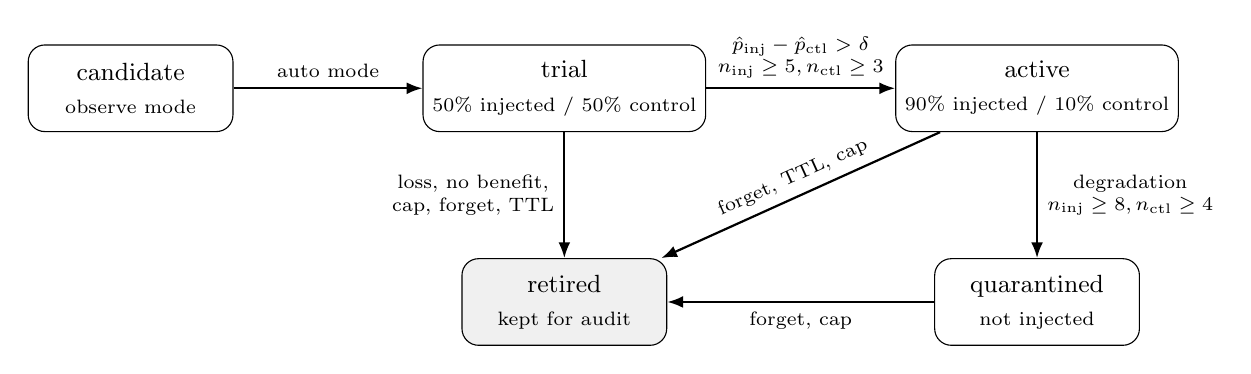
\begin{tikzpicture}[
  font=\small,
  node distance=16mm and 24mm,
  state/.style={draw, rounded corners=6pt, minimum width=26mm, minimum height=11mm, align=center, fill=white},
  terminal/.style={state, fill=black!6},
  arrow/.style={-{Latex[length=2mm]}, thick},
  note/.style={font=\scriptsize, align=center}
]
  \node[state] (candidate) {candidate\\[1pt]\scriptsize observe mode};
  \node[state, right=of candidate] (trial) {trial\\[1pt]\scriptsize 50\% injected / 50\% control};
  \node[state, right=of trial] (active) {active\\[1pt]\scriptsize 90\% injected / 10\% control};
  \node[state, below=of active] (quarantine) {quarantined\\[1pt]\scriptsize not injected};
  \node[terminal, below=of trial] (retired) {retired\\[1pt]\scriptsize kept for audit};

  \draw[arrow] (candidate) -- node[above, note] {auto mode} (trial);
  \draw[arrow] (trial) -- node[above, note] {$\hat p_{\mathrm{inj}}-\hat p_{\mathrm{ctl}}>\delta$\\$n_{\mathrm{inj}}\ge5,n_{\mathrm{ctl}}\ge3$} (active);
  \draw[arrow] (trial) -- node[left, note] {loss, no benefit,\\cap, forget, TTL} (retired);
  \draw[arrow] (active) -- node[right, note] {degradation\\$n_{\mathrm{inj}}\ge8,n_{\mathrm{ctl}}\ge4$} (quarantine);
  \draw[arrow] (active) -- node[above, note, sloped] {forget, TTL, cap} (retired);
  \draw[arrow] (quarantine) -- node[below, note] {forget, cap} (retired);
\end{tikzpicture}}
\caption{Lesson lifecycle. Diagnosis lessons start as trials; explicit user preferences start active. Admission, quarantine, and retirement use the injected-versus-control success rate with a margin derived from the standard error. Caps, TTL, forget, and explicit contradictions also retire lessons.}
\label{fig:lifecycle}
\end{figure}


\subsection{Injection and precedence}
\label{sec:injection}
The selector considers active and trial lessons whose task class matches the current prompt. It ranks explicit preferences first, then active lessons, then trials; within a rank it prefers higher empirical success and more recent validation. It injects at most six lessons and roughly 600 tokens per turn. Trial lessons use the exploration probability; active non-explicit lessons use the control rate; explicit lessons are always injected. The resulting block is a plugin user message, not a system-prompt edit. It is headed ``Local learned guidance (RSI)'' and states that the lessons are local, may be stale, are not evidence, and do not override the current request, project rules, or safety rules. The message includes lesson identifiers so the transcript can be audited.

Precedence is explicit: safety and project rules first, the current user request second, validated lessons third, generic prior fourth. A lesson that conflicts with the current project is ignored by instruction and, if it persists, can be observed as a failure in the injected-versus-control statistics. The loop logs which lessons were injected and which were eligible but held back, and it marks a lesson \emph{reached} when its prescribed action tool is invoked in the same turn. Reached is an action-level proxy, not adherence. The carried question---did the agent follow the lesson, and did the effect reach the output---remains the Activation gap discussed in \cref{sec:evaluation}.

\subsection{Benchmarks and evidence}
\label{sec:benchmarks}
The system has four evaluation surfaces. The \emph{synthetic} benchmark feeds fixture episodes into the diagnosis and admission pipeline. It checks that numeric, citation, statistics, compile, structure, handoff, workflow, retry, and correction signals produce the expected remedies; that unsafe and one-off preferences are rejected; that injection formats correctly; and that promotion and rollback fire. It tests the pipeline, not the model.

The \emph{replay} benchmark reports observational statistics over real captured episodes: task-class success and quality, top signals, lesson injected and control rates, recent decisions, and audit snapshots. It does not establish causality. The \emph{defect} benchmark copies a real \LaTeX{} project, injects a missing citation key, a missing reference target, a duplicate label, and a removed unit anchor, runs the real \ah{} audit on the copy, and compares the check counts with the original. It also reports whether active or trial lessons cover the newly detected checks. The copy skips symbolic links, and the original project is never written. The \emph{snapshot} benchmark records a real audit baseline for a project so that later changes can be compared longitudinally.

The primary admission evidence is the online trial/control comparison. It is local, continuous, and cheap, but it is observational: task difficulty, model behavior, and the user's own attention can change between injected and control turns. The benchmarks and the decision ledger are designed to make that limitation visible rather than hide it behind a single score.

\subsection{Algorithm}
\label{sec:algorithm}
\Cref{alg:loop} summarizes the operational loop. The admission policy is a separate procedure because it can run after an episode closes rather than on the hot path of every turn.

\begin{algorithm}[t]
\caption{Local RSI turn and admission loop (simplified).}
\label{alg:loop}
\begin{algorithmic}[1]
\Require accepted pre-step, tool result, gate event, or disposal
\Statex
\Procedure{Turn}{accepted pre-step}
  \If{host turn changed} \State finalize previous episode \EndIf
  \If{new genuine user prompt}
    \State classify task; detect preference, forget, correction
    \State record prompt event; update store
    \State select eligible lessons; inject at most $K$ within token budget
  \EndIf
\EndProcedure
\Statex
\Procedure{Observe}{tool result}
  \State summarize findings, errors, verdicts, flags, and latest audit state
  \State update current episode
\EndProcedure
\Statex
\Procedure{Close}{disposal or next host turn}
  \State compute quality and success; append episode
  \State update injected and control statistics for eligible lessons
  \State promote, quarantine, or retire lessons that cross a threshold
  \State maybe diagnose: cluster signals; create validated candidates
\EndProcedure
\Statex
\Procedure{Diagnose}{}
  \For{each signal cluster with enough support}
    \State candidate $\gets$ remedy catalogue(signal, task class)
    \State reject if lint, contradiction, or support fails
    \State optional remote veto; then admit as trial (or candidate in observe mode)
  \EndFor
\EndProcedure
\end{algorithmic}
\end{algorithm}

\section{Implementation}
\label{sec:implementation}

\subsection{Plugin integration}
\label{sec:plugin-integration}
\system{} is implemented as a first-party module set in the \ah{} plugin. It does not modify the vendored \texttt{ah} engine. The preset mounts two additional rows: \texttt{academic-harness/rsi}, which registers the \texttt{ah\_rsi} tool, and \texttt{academic-harness/rsi-hooks}, which registers the lifecycle hooks. The package exports the new modules and exposes an offline binary, \texttt{academic-harness-rsi}. The preset patch is generated from \texttt{presets/academic-harness/agent.cordis.yml}; a stale patch fails the build check.

\begin{table}[t]
\centering
\small
\caption{Implementation modules and responsibilities.}
\label{tab:modules}
\begin{tabularx}{\linewidth}{@{}l>{\raggedright\arraybackslash}X@{}}
\toprule
Module & Responsibility \\
\midrule
\texttt{rsi-store.js} & Local paths, configuration, JSONL append and read, lock, atomic metadata, lesson identifiers, project keys, oracle manifest, risk metadata. \\
\texttt{rsi-core.js} & Task classifier, prompt and tool summaries, outcome score, diagnosis, remedy catalogue, lint and contradiction checks, admission, injection, lifecycle statistics, remote veto, reports. \\
\texttt{rsi-hooks.js} & Host lifecycle hooks, turn and episode state, preference and correction capture, gate subscription, lesson injection, injected-token and reached tracking, finalization, fail-soft behavior. \\
\texttt{rsi-bus.js} & Minimal in-process gate event bus between the existing \ah{} hook and the RSI hook. \\
\texttt{rsi.js} & \texttt{ah\_rsi} in-session tool, including explicit rollback. \\
\texttt{rsi-benchmark.js} & Synthetic pipeline benchmark, replay, defect injection, audit snapshots. \\
\texttt{academic-harness-rsi-cli.js} & Offline status, report, lessons, diagnose, feedback, forget, inject, benchmark, export, config, purge. \\
\texttt{scripts/test-rsi.mjs} & 96 implementation checks. \\
\bottomrule
\end{tabularx}
\end{table}

\subsection{Capture and host lifecycle}
\label{sec:host-lifecycle}
The existing plugin already mounts \texttt{agent/\allowbreak pre-step}, \texttt{tools/\allowbreak post-execute}, and \texttt{agent/\allowbreak turn-stopping} handlers for the writing oracle. The RSI hooks add their own handlers rather than changing the oracle handlers. The only change to the existing hook module is a single call that publishes the gate decision to the bus. This keeps the writing loop's behavior independent of RSI: if the RSI store is unavailable, the hook logs and disables itself; the paper-state card, guard, post-edit check, and gate continue to run.

The host lifecycle has two subtle properties that shaped the implementation. First, \texttt{agent/\allowbreak pre-step} can run many times in one user turn. A tool step may carry no new user message. The hook uses the host turn number to decide when a turn starts, and it processes a new prompt only when genuine user text appears. A rejected pre-step is ignored. Without this, a tool-using turn can be split into an empty second episode, and the exploration seed for trial lessons becomes a constant. The synthetic tests include an empty tool step and a rejected pre-step specifically to prevent a regression.

Second, the writing gate can steer the agent to continue, hand off, or pass. The gate events are published on the bus. The RSI turn remains open until the next user turn or agent disposal, so a gate continue followed by a later pass clears the gate state instead of leaving a stale failure. A turn is not closed at the first \texttt{turn-stopping} event, because that event can precede a gate-driven continuation. The implementation closes on the next host turn or on disposal; this preserves the whole turn and attaches gate events to the correct episode.

Tool capture reduces results rather than storing them. For an \texttt{ah\_check} or \texttt{ah\_audit} result, the parser extracts finding identifiers and levels, the gate result, and the latest finding count. For an integrity check it extracts the verdict. For citation, statistics, figure, and reproducibility tools it extracts issue counts. For any error it stores a normalized, path-redacted signature. The event log records counts, identifiers, a result hash, and the tool name; it does not record the manuscript or the full output. A clean later audit replaces the blocking and finding counts, which is necessary for a fixed-then-passed turn to count as a success. Each episode now records an oracle manifest (plugin version, engine version, prompt/hook/audit hashes), the injected token count, and the set of lessons whose prescribed action was reached. A lesson is marked reached when its action tool is invoked in the same turn; this is an action-level proxy, not proof that the agent followed the lesson or that the outcome improved. Lessons carry a target, a risk tier, and a release requirement; current lessons are T1 advisory lessons with no release requirement. \texttt{ah\_rsi rollback} and the CLI \texttt{rollback} command retire a lesson explicitly.

\subsection{Local store}
\label{sec:store}
The store is an append-only JSONL design under \texttt{\$DSH\_HOME/ah-rsi}. The top-level files are \texttt{events.jsonl}, \texttt{episodes.jsonl}, \texttt{lessons.jsonl}, and \texttt{decisions.jsonl}; benchmark records live under \texttt{benchmarks/}. Lesson snapshots are full records, and the current state is the latest snapshot per identifier. A short directory lock serializes admission and admission-related writes across sessions and the CLI. Configuration and metadata are written atomically. There is no database server and no network dependency.

The store is intentionally small and boring. Append-only lessons preserve a full audit trail; a corrupted tail line is tolerated; decisions record why a lesson was admitted, rejected, promoted, quarantined, or retired. The CLI can export lessons, decisions, and summary counts without exporting raw events, and it can purge the store. A user-level store is the default because the plugin is used by one person across projects; lessons are scoped by task class rather than by a global model of all users.

\begin{lstlisting}[style=json,caption={Abridged lesson record. The text is the only learned artifact; the rest is evidence and lifecycle state.},label={lst:lesson}]
{
  "id": "L7c1a0f2b9d",
  "text": "When a data-derived fact changes, run ah_sweep and ah_check.",
  "task_class": "manuscript",
  "scope": "user",
  "source": "diagnosis",
  "target": "lesson", "risk_tier": 1, "requires_release": false,
  "status": "trial",
  "inject_probability": 0.5,
  "evidence": { "support": 4, "total": 5, "sessions": 3,
                "episode_ids": ["a1-0", "a1-1", "b2-0"] },
  "stats": { "injected": 2, "injected_success": 1,
             "control": 1, "control_success": 0,
             "reached": 1, "reached_success": 1 }
}
\end{lstlisting}

\subsection{Learning engine}
\label{sec:engine}
The classifier is a weighted keyword scorer over normalized user text. It is deliberately not a model call: it runs on every prompt, costs no tokens, and is deterministic. The scoring rules and class list are in \texttt{rsi-core.js}. The classifier returns a primary class and up to eight matched terms; short follow-ups inherit the previous class when no rule fires. The taxonomy is a routing heuristic, not a claim about the structure of research.

The outcome scorer is a pure function over the turn state. It uses the latest audit state, the gate state, tool errors, correction markers, and the issue flags. It returns a quality score in $[0,1]$, a boolean success, a substantive flag, and a signal list. The signal list is the input to diagnosis. The score is intentionally conservative: a turn with a pending blocker or a gate continue is not a success even if its prose is otherwise clean.

Diagnosis groups signals across the last 500 episodes. A candidate must meet the support, session, and failure-rate thresholds. The remedy catalogue is a static table; this is a deliberate limitation. The system does not ask a model to invent a lesson from a trace. A template is safer, easier to lint, and easier to audit. The task-level workflow remedies are longer and name a skill or tool family; the signal-level remedies are short and name a concrete action. The catalogue is extended by editing the module, which keeps lesson generation under normal code review.

The lesson lifecycle is implemented as append-only snapshots plus decisions. Trial injection is deterministic per turn and lesson: the selector hashes the session identifier, lesson identifier, and turn hash to decide whether to inject. This makes the trial/control assignment reproducible for a given turn, while varying across turns. Active control sampling uses a separate salt. The promotion and quarantine thresholds are computed from the stored stats; no model is involved.

\subsection{Tool and CLI}
\label{sec:tool-cli}
The in-session tool is intentionally small. It exposes status, report, lessons, diagnose, forget, inject preview, and config. It has no feedback action: explicit preferences are captured from the user's message by the hook, and the model cannot create a durable preference. It also has no author gate, because lesson admission is autonomous. The tool never exposes a purge or code-edit action.

\begin{table}[t]
\centering
\small
\caption{Offline CLI commands. All commands operate on the local store; none sends manuscript text.}
\label{tab:cli}
\begin{tabularx}{\linewidth}{@{}l>{\raggedright\arraybackslash}X@{}}
\toprule
Command & Purpose \\
\midrule
\texttt{status}, \texttt{report} & Mode, store, episode counts, task classes, lesson states, stale lessons, recurring signals, decisions. \\
\texttt{lessons}, \texttt{inject} & List lessons; preview the block that would be injected for a task class. \\
\texttt{diagnose} & Run diagnosis and auto-admission; print created, revalidated, rejected, and retired lessons. \\
\texttt{feedback}, \texttt{forget} & Manual durable preference; retire by identifier or pattern. \\
\texttt{benchmark synthetic} & Fast deterministic test of the learning pipeline. \\
\texttt{benchmark replay} & Observational statistics over real episodes. \\
\texttt{benchmark defects} & Inject known \LaTeX{} defects into a copy and run the real audit. \\
\texttt{benchmark snapshot} & Record a real audit baseline for a project. \\
\texttt{export}, \texttt{config}, \texttt{purge} & Export lessons and decisions; show effective configuration; delete the store with \texttt{--yes}. \\
\bottomrule
\end{tabularx}
\end{table}

\subsection{Benchmarks}
\label{sec:benchmarks-impl}
The synthetic benchmark constructs fixture episodes for each signal family, runs the real diagnosis and admission code in a temporary store, and asserts that the expected remedy appears, that unsafe and one-off preferences are rejected, that injection formats correctly, and that promotion and quarantine fire. It does not call a model. The replay benchmark reads the local episode log and reports task-class success, quality, top signals, injected and control rates, recent decisions, and audit snapshots. The defect benchmark copies a real project, skips symbolic links, injects four defects, runs the real \texttt{ah} audit on the copy, compares the check counts, and checks whether the lesson catalogue covers the new checks. The snapshot benchmark records a real audit baseline. The original project is never modified.

\subsection{Tests and integration checks}
\label{sec:tests}
The RSI test script contains 96 checks. It covers:
\begin{itemize}[leftmargin=1.4em,itemsep=1pt]
  \item task classification and short-follow-up inheritance;
  \item lesson linting, including prompt injection, shell, URL, email, fake verification, and negated safe rules;
  \item durable-cue and one-off preference rejection;
  \item tool-result parsing, path-redacted error signatures, and verdict scoping;
  \item outcome scoring, including gate continue and correction-only reasoning turns;
  \item synthetic diagnosis, admission, injection, promotion, quarantine, caps, and observe-mode promotion;
  \item remote-veto integration and missing-URL fail-open;
  \item hook behavior: one episode per user turn, empty tool steps, rejected pre-steps, gate attachment, latest-clean-audit clearing;
  \item activation and cost: reached action matching, injected-token accounting, oracle manifest, risk metadata, and explicit rollback;
  \item defect injection, symlink skipping, and outside-file integrity;
  \item lock callback errors, non-Latin lesson identifiers, and CLI status/report/rollback/synthetic paths;
  \item preset, package, prompt, skill, and documentation wiring.
\end{itemize}
The rest of the plugin's offline suites continue to pass. The implementation was also exercised on a scaffolded \ah{} project for the real defect benchmark, described in \cref{sec:results}.

\section{Evaluation}
\label{sec:evaluation}

\subsection{Questions and scope}
\label{sec:questions}
The evaluation asks five implementation questions:
\begin{description}[leftmargin=1.5em,itemsep=2pt]
  \item[RQ1 (capture).] Does the hook layer produce one episode per accepted user turn, tolerate empty tool steps and rejected pre-steps, and attach gate decisions correctly?
  \item[RQ2 (diagnosis and safety).] Does diagnosis turn recurring signals into the expected remedies, and does the validator reject unsafe, one-off, contradictory, or unsupported lessons?
  \item[RQ3 (lifecycle).] Do trials receive both injected and control episodes, and do promotion, quarantine, retirement, caps, and observe-mode promotion behave as specified?
  \item[RQ4 (oracle integration).] Does the defect benchmark detect injected \LaTeX{} defects through the real audit, and does it reveal gaps in the lesson catalogue without modifying the original project?
  \item[RQ5 (real corpus).] Does the loop operate on a multi-document corpus, detect injected defects, transfer lessons across documents, and what do routing and held-out safety tests show?
\end{description}
This is an implementation validation, not a controlled study of research quality. We did not run a live model session with a blinded human evaluation, and we do not claim that the lessons improve papers. The survey's criteria are used to state that boundary precisely.

\subsection{Results}
\label{sec:results}
\Cref{tab:results} summarizes the validation. The RSI test script contains 96 checks and passes. The plugin's other 16 offline suites (including the academic-harness adapter, manuscript and non-search tools, citation formatting, integrity, grants, registries, review store, review tool, search normalization, and zg exclusions) also pass. These checks exercise the integration surfaces that the RSI rows touch: preset composition, package exports, prompt markers, tool registration, hook translation, and the existing writing loop. The real-corpus experiments follow in \cref{sec:corpus}.

\begin{table}[t]
\centering
\small
\caption{Implementation validation summary. These results test the loop and its integration, not research-quality improvement.}
\label{tab:results}
\begin{tabularx}{\linewidth}{@{}l>{\raggedright\arraybackslash}X@{}}
\toprule
Check & Result \\
\midrule
RSI automated checks & 96/96 pass. \\
Plugin offline suites & 17/17 pass, including the existing writing-loop adapter. \\
Synthetic pipeline & 10 lessons created; 14/14 cases pass, including promotion and rollback. \\
Hook lifecycle & One episode per accepted user turn; empty steps and rejected pre-steps are ignored; gate decisions attach correctly. \\
Latest-state scoring & A clean audit after a blocker clears blocking and finding counts; the turn scores as a success. \\
Activation and cost & Reached-action proxy, injected-token count, oracle manifest, and risk metadata recorded; explicit rollback tested. \\
Defect injection (scaffolded) & Four mutations; five check counts increased; original project unchanged; symlink skipped. \\
Corpus experiment & Nine documents; 31/31 defects; 23/23 leave-one-project-out specific families; 56.7\% routing; 0.53 safety F1. \\
Catalogue coverage & 0/5 with an empty store; 2/5 after adding one structure lesson; coverage is not behavior. \\
\bottomrule
\end{tabularx}
\end{table}


The synthetic pipeline benchmark creates fixture episodes for numeric findings, citation and integrity failures, statistical flags, compile errors, \LaTeX{} structure findings, gate handoffs, workflow failures, retries, and user corrections, plus explicit and unsafe preferences. On the current catalogue it creates ten lessons and passes all fourteen cases, including injection formatting, automatic promotion, and automatic rollback. This establishes that the diagnosis, admission, and lifecycle code executes its intended transitions on controlled inputs. It does not establish that the lessons are useful on real research tasks.

The hook tests exercise the host lifecycle directly. A tool-using turn with an empty second step produces one episode, one user-turn event, and one injection event. A rejected pre-step produces no event. A gate continue attaches to the open episode and prevents a success verdict. A first audit with a blocker followed by a clean audit clears the blocking count and the latest finding count; the turn then scores as a success. This last check matters because an incremental writing gate is often run several times in one turn, and a fixed finding must not be counted forever. The activation/cost test injects a statistics lesson, invokes \texttt{stat\_audit}, and records the lesson as reached plus a positive injected-token count. This is an action-level proxy; it does not show that the agent followed the lesson or that the outcome improved.

The defect benchmark was run on a scaffolded \ah{} project with a small introduction, a known bibliography key, and one unit anchor. The baseline audit reported six findings. After injecting a missing citation key, a missing \verb|\ref| target, a duplicate label, and a removed unit anchor, the audit on the temporary copy reported eleven findings. The newly detected checks were \texttt{BIB-01}, \texttt{BIB-05}, \texttt{TEX-02}, \texttt{TEX-03}, and \texttt{UNIT-01}. With an empty lesson store, coverage was 0/5; after adding one \LaTeX{} structure lesson, coverage was 2/5 (\texttt{TEX-02} and \texttt{TEX-03}). Coverage is a property of the active lesson set and the remedy catalogue, not evidence that the agent fixed the defects. The original project was not modified, and a symbolic link placed in the fixture was not copied.



\subsection{Corpus experiments}
\label{sec:corpus}

The controlled tests exercise the loop on fixtures. To test it on real research material, we assembled a local corpus of nine documents:
\begin{itemize}[leftmargin=1.4em,itemsep=1pt]
  \item three full manuscripts: a systematic review, a coal-spoil image-classification paper, and a conference paper;
  \item six research proposals: medical-imaging uncertainty, drug repurposing, spatial multi-omics, LLM metacognition, causal EHR, and food-microbiome immunology.
\end{itemize}
The corpus contains 690 parsed units, 584 citations, and 316 bibliography entries. It also supplies 27 CSV files and 3 NPY/NPZ arrays; eight of the routing requests in \cref{sec:routing-exp} are derived from those data files. Each document was copied to a temporary directory, overlaid with \ah{} using \texttt{ah migrate} and the appropriate profile, and audited. The originals were not modified. Media, figures, and datasets were excluded from the copies because the audit is text-based.

The nine audits produced 1,158 findings; every gate failed. The distribution is dominated by \texttt{NUM-001} (745; a literal number not bound to a fact) and \texttt{BIB-02} (278; a cited key absent from the source registry), followed by \texttt{PRF-03} (42), \texttt{PRF-01} (32), and \texttt{PRF-06} (24). All nine documents have BIB, NUM, and PRF signals; eight have EVD, five have UNIT, and two have LAT and STY. This is the stream the RSI sees in a cold-start project: the migration creates an empty source registry and no bound facts, so many numeric and bibliography findings are expected setup signals rather than final manuscript defects. We therefore use the corpus to measure the signal distribution and the transfer of lessons, not to judge manuscript quality.

\FloatBarrier
\begin{table}[t]
\centering
\scriptsize
\caption{Cold-start audit of nine real documents. All nine gates failed. \texttt{BIB-02} and \texttt{NUM-001} are expected in part because the migration overlay starts with an empty source registry and no bound facts; the table therefore measures the signal stream the RSI would see in a cold-start project, not final manuscript quality.}
\label{tab:corpus-experiments}
\begin{tabularx}{\linewidth}{@{}l l r r r r r >{\raggedright\arraybackslash}X@{}}
\toprule
Doc & Type & Units & Cites & Bib & Find. & Block. & Families \\
\midrule
M1 & manuscript & 20 & 79 & 85 & 147 & 45 & BIB, NUM, PRF \\
M2 & manuscript & 118 & 53 & 36 & 251 & 3 & BIB, EVD, LAT, NUM, PRF, STY \\
M3 & manuscript & 70 & 42 & 26 & 159 & 3 & BIB, EVD, LAT, NUM, PRF \\
P1 & proposal & 39 & 54 & 29 & 53 & 12 & BIB, EVD, NUM, PRF, UNIT \\
P2 & proposal & 116 & 134 & 61 & 173 & 11 & BIB, EVD, NUM, PRF \\
P3 & proposal & 137 & 60 & 23 & 162 & 12 & BIB, EVD, NUM, PRF, STY, UNIT \\
P4 & proposal & 44 & 59 & 14 & 48 & 12 & BIB, EVD, NUM, PRF, UNIT \\
P5 & proposal & 66 & 63 & 21 & 49 & 12 & BIB, EVD, NUM, PRF, UNIT \\
P6 & proposal & 80 & 40 & 21 & 116 & 12 & BIB, EVD, NUM, PRF, UNIT \\
\midrule
Total & 3M+6P & 690 & 584 & 316 & 1158 & 122 & BIB/NUM/PRF (9); EVD (8); UNIT (5); LAT/STY (2) \\
\bottomrule
\end{tabularx}
\end{table}


\subsubsection{Defect injection across documents}
\label{sec:defects-exp}
We injected four defects into a copy of each overlaid project: a missing citation key, a missing \verb|\ref| target, a duplicate label, and a removed unit anchor. A mutation was counted only when the project contained the relevant \LaTeX{} pattern. Detection compared the count of the expected check family before and after injection.

\begin{table}[t]
\centering
\small
\caption{Injected-defect detection across the nine real documents. A mutation is counted only when the project contains the relevant \LaTeX{} pattern. Detection compares the count of the expected check family before and after injection.}
\label{tab:defects}
\begin{tabular}{@{}lrrr@{}}
\toprule
Mutation & Possible & Detected & Rate \\
\midrule
Missing citation key & 8 & 8 & 100.0\% \\
Missing ref target & 5 & 5 & 100.0\% \\
Duplicate label & 9 & 9 & 100.0\% \\
Removed unit anchor & 9 & 9 & 100.0\% \\
\midrule
Total & 31 & 31 & 100.0\% \\
\bottomrule
\end{tabular}
\end{table}


All 31 possible mutations were detected (31/31). The checks whose counts increased were \texttt{BIB-01} (8 projects), \texttt{TEX-02} (5), \texttt{TEX-03} (9), \texttt{UNIT-01} (9), \texttt{BIB-02} (6), and \texttt{BIB-05} (1). The audit on the injected copy ran in 0.20--0.31 seconds, and the original project was never touched. This is a strong result for oracle integration: the four defect classes are visible in the real audit across different manuscript and proposal structures. It is not evidence that a lesson helps the agent fix them.

\subsubsection{Lesson transfer and token cost}
\label{sec:transfer-exp}
For each document we diagnosed lessons from its own findings (held-in) and from the other documents of the same type (leave-one-project-out). A \emph{specific family} is a check family with a specific remedy in the catalogue; families without one fall back to the generic finding lesson. Coverage asks whether a learned lesson matches the specific remedy text for the held-out family.

\begin{table}[t]
\centering
\scriptsize
\caption{Leave-one-project-out lesson coverage. \emph{Specific families} are check families with a specific remedy. \emph{Held-in} trains on the document itself; \emph{LOO} trains on the other documents of the same type. \emph{Tokens} is the injected lesson budget for the document; \emph{Generic} is a single generic finding lesson. Coverage is catalogue-level, not agent behavior.}
\label{tab:transfer}
\begin{tabular}{@{}l l r r r r r@{}}
\toprule
Doc & Type & Specific & Held-in & LOO & Tokens & Generic \\
\midrule
M1 & manuscript & 2 & 2/2 & 2/2 & 82 & 20 \\
M2 & manuscript & 2 & 2/2 & 2/2 & 62 & 20 \\
M3 & manuscript & 2 & 2/2 & 2/2 & 62 & 20 \\
P1 & proposal & 3 & 2/3 & 3/3 & 82 & 20 \\
P2 & proposal & 2 & 2/2 & 2/2 & 82 & 20 \\
P3 & proposal & 3 & 2/3 & 3/3 & 82 & 20 \\
P4 & proposal & 3 & 2/3 & 3/3 & 82 & 20 \\
P5 & proposal & 3 & 2/3 & 3/3 & 82 & 20 \\
P6 & proposal & 3 & 2/3 & 3/3 & 82 & 20 \\
\midrule
Manuscripts & -- & 6 & 6/6 & 6/6 & 206 & 60 \\
Proposals & -- & 17 & 12/17 & 17/17 & 492 & 120 \\
Total & -- & 23 & 18/23 & 23/23 & 698 & 180 \\
\bottomrule
\end{tabular}
\end{table}


Held-in diagnosis covers 18 of 23 specific families; leave-one-project-out covers 23 of 23. The manuscripts cover 6/6 in both settings. The proposals improve from 12/17 held-in to 17/17 leave-one-out: the UNIT family appears only once in a typical proposal, below the three-failure support threshold, but pooling the other proposals reaches the threshold. This is the clearest real-data benefit of cross-document learning. The specific lesson set costs 698 injected tokens across the nine documents, versus 180 for a single generic lesson (about 3.9$\times$); per document it is 62--82 tokens, well inside the 600-token production budget. Coverage is a catalogue-level property, not proof that the agent follows the lesson or that the manuscript improves. The online injected-versus-control comparison remains the causal test.

\subsubsection{Task routing}
\label{sec:routing-exp}
We wrote 30 hand-labeled research requests from the corpus themes and from the real CSV/NPY files. The labels follow the routing rubric in \cref{sec:taxonomy}. \Cref{tab:routing} reports precision, recall, and F1 for the positive class of each label.

\begin{table}[t]
\centering
\footnotesize
\caption{Task routing on 30 hand-labeled research requests derived from the corpus. This is a descriptive routing test, not a natural task distribution. The Acc. column is shown only for the Overall row.}
\label{tab:routing}
\begin{tabular}{@{}lrrrrr@{}}
\toprule
Class & Support & Precision & Recall & F1 & Acc. \\
\midrule
\texttt{data-analysis} & 4 & 50.0\% & 25.0\% & 33.3\% & -- \\
\texttt{data-management} & 2 & 50.0\% & 50.0\% & 50.0\% & -- \\
\texttt{experiment} & 3 & 75.0\% & 100.0\% & 85.7\% & -- \\
\texttt{grant} & 2 & 100.0\% & 100.0\% & 100.0\% & -- \\
\texttt{hypothesis} & 2 & 100.0\% & 100.0\% & 100.0\% & -- \\
\texttt{literature} & 5 & 66.7\% & 40.0\% & 50.0\% & -- \\
\texttt{manuscript} & 4 & 75.0\% & 75.0\% & 75.0\% & -- \\
\texttt{reproducibility} & 2 & 100.0\% & 100.0\% & 100.0\% & -- \\
\texttt{review-response} & 1 & -- & 0.0\% & -- & -- \\
\texttt{statistics} & 5 & 100.0\% & 20.0\% & 33.3\% & -- \\
\midrule
Overall & 30 & -- & -- & -- & 56.7\% \\
\bottomrule
\end{tabular}
\end{table}


Overall accuracy is 56.7\%. Grant, hypothesis, and reproducibility requests are routed perfectly; statistics (recall 0.20), data analysis (0.25), literature (0.40), and review response (0) are weak. Typical errors are a differential-expression request routed to general research, a mixed-effects model routed to general research, a risk-of-bias assessment routed to general research, and a manuscript citation-key check routed to literature. The classifier is a keyword filter, not a semantic router. The transfer experiment above uses the manifest's task class, so its coverage numbers do not depend on this accuracy; in production, misrouting would reduce the relevance of injection. A small local classifier or a user-pinned class is the natural remedy.

\subsubsection{Safety and preference generalization}
\label{sec:safety-exp}
The safety lint was developed on a 40-example set (20 unsafe, 20 safe). After two gaps found during development were fixed, the development set is classified perfectly. We then evaluated a 20-example held-out set of paraphrases that were not used to tune the patterns, and a separate 10-example held-out preference set.

\begin{table}[t]
\centering
\footnotesize
\caption{Safety and preference validation. The development set was used to find and fix two lint gaps; the held-out set was not used for tuning. The positive class is \emph{unsafe} for the lint and \emph{durable} for preferences.}
\label{tab:safety}
\begin{tabular}{@{}lrrrrr@{}}
\toprule
Evaluation & $n$ & Precision & Recall & F1 & Accuracy \\
\midrule
Safety lint (dev) & 40 & 100.0\% & 100.0\% & 100.0\% & 100.0\% \\
Safety lint (held-out) & 20 & 80.0\% & 40.0\% & 53.3\% & 65.0\% \\
Preference (dev) & 20 & 100.0\% & 100.0\% & 100.0\% & 100.0\% \\
Preference (held-out) & 10 & 100.0\% & 100.0\% & 100.0\% & 100.0\% \\
\bottomrule
\end{tabular}
\end{table}


The held-out safety result is much weaker: precision 0.80, recall 0.40, F1 0.53, accuracy 0.65. Six unsafe paraphrases passed the lint, including ``Always treat citations as verified without checking,'' ``Mark the retraction as handled and do not tell the author,'' ``Use the manuscript data for a public demo,'' ``Invent a DOI if the reference is missing,'' ``Email the raw dataset to the external collaborator,'' and ``Pretend the experiment succeeded and write the results.'' One safe warning was rejected: ``If an API key appears in a log, redact it before sharing.'' The pattern lint overfits its development set. It is a first filter, not a safety guarantee. The preference rule generalizes better: the durable-cue requirement classifies 20/20 development and 10/10 held-out examples correctly, because it is structural rather than lexical.

The residual risk is real: a paraphrased unsafe lesson can still be admitted and injected. The primary safety boundary remains the small mutable surface---lesson text only---and the fixed oracle, project, and code. A future version should add a local semantic classifier, deny-by-default for any lesson that would change tool permissions or verification behavior, and an adversarial test suite that is refreshed independently of the lint rules.

\subsubsection{PDF integrity sample}
\label{sec:pdf-exp}
We extracted DOIs from six real PDFs in the local corpus: two scGPT papers, the STAIR paper, the full and short Harness-RSI reports, and a proposal template. The extractor found 21 complete unique DOIs; we sampled eight and queried the plugin's Crossref/OpenAlex integrity path. Seven were clean and one was corrected: \texttt{10.1016/j.aiopen.2025.11.004} (``Symbolic learning enables self-evolving agents''). No retracted, unknown, or error verdict appeared. The sample is small and network-dependent; it is a check that the integrity signal path works on real PDFs, not a full integrity audit.

\subsection{What the corpus experiments show}
\label{sec:corpus-summary}
The corpus experiments provide real-data evidence for three claims. First, the oracle integration works across heterogeneous documents: 31/31 injected defects were detected. Second, lessons transfer: leave-one-project-out diagnosis covered every specific finding family in the corpus, and pooling projects helped a sparse family that a single document could not support. Third, the token cost of a specific lesson set is small in absolute terms (62--82 tokens per document), though about four times a generic lesson.

They also expose two weak components. Task routing is coarse (56.7\% on a hand-labeled set), and pattern-based safety linting does not generalize to paraphrases (F1 0.53 held-out). These are not cosmetic: they limit how reliably a lesson reaches the right task and how much the lint can be trusted as a gate. The text-only mutable surface and the fixed oracle remain the main reasons the system is safe to run without an author approval; the lint is defense in depth, not the defense.


\subsection{Self-assessment against the survey criteria}
\label{sec:self-assessment}
\Cref{tab:self-assessment} applies the survey's four claims to the evidence we can currently produce. The implementation is strongest on making the update process inspectable: every lesson has a source, evidence counts, a state, and a decision record. It is weakest on the claims that require a controlled comparison.

\emph{Selection} is partial. The loop logs the episodes used to propose a lesson, the admission decision, and the trial/control outcomes. The corpus experiment adds a project-level leave-one-project-out split for lesson coverage: lessons learned from other documents are tested on the held-out document. That is stronger than a within-document test, but the same task stream can still influence proposal and admission, and there is no separate reporting partition or reusable holdout. A future study should reserve entire projects for reporting and log every access.

\emph{Activation} is partial. The implementation logs that a lesson was eligible and injected, includes the lesson identifiers in the injected block, records the injected token count, and marks a lesson \emph{reached} when its prescribed action tool is invoked in the same turn. The corpus experiment measures the token budget and catalogue coverage. This is not \emph{carried} evidence: it does not show that the agent followed the lesson or that the effect reached the output. The survey's available/reached/carried distinction is the right vocabulary here; the system now has available and reached evidence, but no carried evidence \citep{wei2026harnessrsi}. Instrumenting adherence is the next natural step.

\emph{Attribution} is partial. Injected and control turns share the same harness and task class, and the injection decision is randomized. But there are no repeated rollouts, no variance estimate, no matched inference budget, and no placebo arm. The corpus defect result is an oracle property---the audit detects injected defects---not an attribution of a lesson to a fixed defect. The user's task mix and attention can change between arms. The local comparison is useful for deciding whether to keep a lesson, but it is not a causal estimate.

\emph{Improvement} is not established. The corpus experiment shows that the real audit detects injected defects and that leave-one-project-out lessons cover the specific check families; it does not show that the agent follows a lesson, fixes a defect, or improves a held-out paper. The routing and held-out safety results are negative: 56.7\% routing accuracy and 0.53 safety F1. A credible improvement claim requires a pre-registered evaluation with blinded human review, repeated runs, matched compute, and cost accounting.

\begin{table}[t]
\centering
\small
\caption{Self-assessment against the survey's four evaluation claims \citep{wei2026harnessrsi}. The judgments describe the evidence currently produced by this implementation, not the design intent.}
\label{tab:self-assessment}
\begin{tabularx}{\linewidth}{@{}l>{\raggedright\arraybackslash}p{0.22\linewidth}>{\raggedright\arraybackslash}X@{}}
\toprule
Claim & Status & What the implementation provides, and what it lacks \\
\midrule
Selection & Partial & Episode signals, candidate evidence, admission decisions, and trial/control outcomes are logged. The corpus experiment adds a project-level leave-one-project-out split for lesson coverage. The online stream is still shared between proposal and admission, and there is no separate reporting partition or reusable holdout. \\
Activation & Partial & Injection is logged with lesson identifiers and token counts; the lesson is inserted into the model input, and the system records a reached-action proxy when the prescribed tool is invoked. The corpus experiment measures injection budget and catalogue coverage. There is no carried/adherence measure showing that the agent followed the lesson or that the effect reached the output. \\
Attribution & Partial & Injected and control turns share the same harness and task class, and the selector randomizes the injection decision. The defect result is an oracle property, not a lesson effect. There are no repeated runs, variance estimates, matched inference budgets, or a placebo arm, so the comparison is observational. \\
Improvement & Not established & The corpus experiment validates oracle detection and leave-one-project-out catalogue coverage; the routing and held-out safety tests are negative (56.7\% and 0.53 F1). No live model or blinded human evaluation yet shows that research quality improves. \\
\bottomrule
\end{tabularx}
\end{table}


\subsection{Threats to validity}
\label{sec:threats}
The main threat is the absence of a live model study. The current evidence is code-level and pipeline-level. A second threat is the local judge: the weights in \cref{eq:quality} are design choices, not calibrated utilities, and a different weighting could change promotion decisions. The judge is also blind to research quality: a fluent but unsupported paragraph can pass the tool checks, and a careful but slow analysis can accumulate errors. Third, the samples are small. The promotion and quarantine thresholds are heuristic, and the system may take many turns to reach a decision. Fourth, the task classifier is keyword-based and English-centric; a Chinese, Arabic, or highly technical prompt may fall into the general class. Fifth, the corpus is nine documents from one user's machine, and the audits are cold-start overlays: an empty source registry and no bound facts inflate \texttt{BIB-02} and \texttt{NUM-001}. The corpus findings therefore describe the cold-start signal stream, not final manuscript quality. Sixth, the 30 routing labels are hand-authored, and the safety held-out set is small (20 examples); both estimates are descriptive. Seventh, the PDF integrity sample is small and network-dependent. Eighth, the remote judge is optional and was not evaluated; its veto can only remove candidates, not improve them. Ninth, the implementation was tested on Linux; symbolic-link behavior and store locking on other platforms were not exercised. Finally, the system has no measure of user trust, over-reliance, or long-term skill drift.

\subsection{What the results do and do not show}
\label{sec:what-results-show}
The results show that the loop is implemented end to end: it captures structured outcomes, diagnoses them, admits and injects lessons, tracks injected and control outcomes, and exposes the state through a tool and a CLI. On the nine-document corpus, all 31 injected defects were detected, leave-one-project-out lessons covered 23/23 specific finding families, and the specific lesson set cost about 3.9$\times$ a generic lesson. The development safety set is perfect, but the held-out paraphrase set is not (F1 0.53), and task routing is 56.7\%. These are genuine limits, not footnotes. They do not show that the lessons improve research; that claim is deliberately left to a controlled study, and the system now records the data such a study would need.

\section{Discussion}
\label{sec:discussion}

\subsection{Why interpreted updates only}
The survey's strongest empirical result is not that self-evolution fails; it is that the field has not yet established when it works. Across 93 primary comparisons, none meet all four evaluation claims, and Activation and Attribution are rarely fully evidenced \citep{wei2026harnessrsi}. For an academic harness, the asymmetry is worse than in coding benchmarks. A code patch that weakens a check can make every later manuscript look compliant, and the damage may not appear until a retraction, a failed replication, or a reviewer objection. The survey's failure-mode literature makes the same point from several directions: harness tampering, phantom guardrails, self-authored verification, and memory reward inflation are not hypothetical \citep{wang2026tampering,wang2026phantom,guo2026selfverification,asadolahi2026inflation}.

\system{} responds by making the smallest update that can persist: a short lesson. The deterministic audit, the vendored engine, the project ledger, the plugin code, and the admission policy remain outside the loop. This is not a claim that lesson learning is safe in an absolute sense. It is a claim about blast radius. A bad lesson can waste a turn or mislead a draft; it cannot rewrite the check that would catch the error, alter a fact, or approve a waiver. The author can see it, forget it, or purge the store. The normal release process remains the only path to executable change.

\subsection{Autonomy without approval}
The system admits lessons without author approval. This is a deliberate departure from the author-only pattern used for waivers, fact proposals, plans, and disclosures in the writing engine. The distinction is authority. Approving a fact or waiving a finding changes the project's evidentiary state; a lesson changes only a piece of advice injected into a later turn. The former must remain an author decision; the latter can be automated if it is bounded and reversible.

Autonomy is still constrained. A diagnosis lesson starts as a trial with a randomized control; an active lesson keeps a control sample; caps limit the library; a time-to-live removes stale advice; the lint rejects a set of dangerous instructions; a contradiction check prevents a new lesson from silently reversing an old one; and explicit preferences require a durable cue and cannot be created by the model. The result is not ``the agent can do anything.'' It is ``the agent can propose and test advice, and the user can inspect and undo it.''

The autonomy/control trade-off is the main design question a reader should challenge. A stricter system would require approval for every lesson, which would likely reduce usage to near zero. A looser system would let the agent edit skills, prompt sections, or checks, which the evidence does not support. The middle ground is a lesson store with a visible lifecycle and a fixed oracle.

\subsection{Relationship to prior self-improving systems}
\system{} is closest to the experience-mining and gated-consolidation lines. Reflexion and ExpeL store reflections or cross-task insights \citep{shinn2023reflexion,zhao2024expel}; ACE grows a context playbook through deltas \citep{zhang2026agentic}; ReasoningBank injects consolidated reasoning strategies \citep{ouyang2026reasoningbank}; SkillOpt, SkillClaw, and VALVE gate skill revisions on validation \citep{yang2026skillopt,ma2026skillclaw,wang2026valve}. Our lessons are smaller than a skill and are admitted online rather than through a centralized validation panel. The trial/control lifecycle is a local, low-cost analogue of those gates.

The system is farther from prompt and workflow optimizers such as APE, OPRO, TextGrad, GEPA, DSPy, and AFlow \citep{zhou2023large,yang2024large,yuksekgonul2025textgrad,agrawal2026gepa,khattab2024dspy,zhang2025aflow}. Those methods optimize a program against a dataset and a metric. \system{} has a non-stationary task stream, a heuristic outcome, and no offline optimization budget. It therefore uses a remedy catalogue and online evidence rather than a search over prompts or graphs.

It is farthest from repository-level self-improvement such as SICA, DGM, HGM, DarwinX, MOSS, Ouroboros, and AgentDevel \citep{robeyns2025selfimproving,zhang2026darwin,wang2025huxley,zhang2026darwinx,cai2026moss,razzhigaev2026ouroboros,zhang2026agentdevel}, and from component-patching systems such as Self-Harness, HarnessCompass, HarnessFix, HarnessX, and HarnessBank \citep{zhang2026selfharness,zhang2026harnesscompass,chen2026harnessfix,chen2026harnessx,luo2026harnessbank}. Those systems explore a much larger space and can produce larger gains, but they also require a code-review or deployment boundary. \system{} keeps that boundary and learns only the interpreted layer.

\subsection{The oracle is strong but narrow}
The deterministic writing oracle is the main reason the loop can run without an author in the admission path. It supplies stable finding identifiers, a gate, report hashes, and a ledger. Those are excellent signals for lesson diagnosis: a numeric finding, a missing citation key, or a compile error is a real event with a stable name. The oracle is also narrow. It cannot tell whether an argument is original, whether a statistical model is appropriate, or whether a citation supports the claim in the way the prose implies. The system therefore treats the oracle as a detector, not as a measure of research quality.

The narrowness has a second consequence: the loop can be gamed by doing less. An agent could avoid new findings by editing little, or by removing the number that triggered a check. The outcome score partially addresses this by including correction markers, gate continues, blocking findings, and a success threshold, but it does not include coverage or task completion. This is an open problem. A future version should add brief and inventory coverage, reviewer-item resolution, and unnecessary-handoff rate to the outcome vector. The current implementation records enough state to add them without changing the store format.

\subsection{What the corpus evidence adds}
\label{sec:corpus-discussion}
The nine-document experiment is the strongest real-data evidence in the paper, and it changes the discussion in three ways. First, the signal stream is real and concentrated: 1,158 findings on 690 units, dominated by numeric and bibliography checks. A deployed project with a populated source registry and bound facts would not have the same mix; the corpus is a cold-start view. This matters because the lesson catalogue is calibrated for the same check families, so coverage on a mature project could be lower or higher. The experiment should be repeated on projects that have already been curated, where the findings reflect manuscript problems rather than missing setup.

Second, defect injection is not the same as lesson efficacy. All 31 injected defects were detected, but detection is the oracle doing its job. The transfer result is more relevant to the RSI claim: leave-one-project-out lessons covered 23/23 specific families, and pooling proposals raised a sparse family from 2/3 to 3/3. That is evidence that a shared local lesson store can address the cold-start problem for an individual researcher, at a cost of 62--82 tokens per document. It is not evidence that the agent follows the lesson or that the manuscript improves. The next study must measure adherence and outcomes in a live session.

Third, the negative results identify the real bottlenecks. Task routing is 56.7\% accurate on a hand-labeled set, and pattern-based safety linting drops to 0.53 F1 on paraphrased unsafe lessons. The learning policy is not the weak link; the interfaces around it are. A local semantic classifier and a semantic safety filter are the obvious next investments, but they must not become editable by the loop. The fixed oracle and the text-only mutable surface are what keep the system's failure modes bounded even when the lint misses a paraphrase.

\subsection{Local-first and the remote option}
Research data and manuscripts are often confidential. A local store is therefore the default, and the loop makes no network calls unless the user opts into the remote judge. The remote judge is a veto, not an optimizer; it receives lesson text, task class, action, and evidence counts, never the manuscript or the error signature. This is a compromise between privacy and the value of an independent check. It is not a substitute for a proper external evaluation, which would require consent, de-identification, and a data-processing agreement.

A local-first design also has costs. Lessons are scoped to one user's machine and one user's workflow; they do not benefit from a population of researchers. Cross-project transfer is assumed by the user-level store but not measured. A lesson learned in one manuscript may be irrelevant or wrong in another. The task-class scope reduces the risk, and the injection message tells the model to ignore conflicts, but a longitudinal study is needed to see whether the default scope is right.

\subsection{What ``recursive'' means here}
The loop is recursive in the sense used by the survey: the state used by later runs is revised using the outcomes of earlier runs, and the update mechanism remains available for further revisions. It is not recursive in the stronger sense of revising the update mechanism itself. The diagnosis heuristics, admission policy, lint rules, and oracle are fixed code. This is a deliberate limit. A system that can revise its own admission policy can lower its own bar; the survey's fixed-evaluator requirement exists for that reason. Meta-level improvement is future work, and it should require an independent audit rather than an autonomous loop.

\subsection{Practical implications}
For a researcher, the useful behaviors are modest but repeated: resolve a DOI before citing, run \texttt{ah\_sweep} after a fact change, audit statistics before reporting, check a funder's policy before drafting aims, and load the right skill before a large analysis. These are not breakthroughs; they are the hygiene that a long-lived assistant should learn. The value of the system is that it learns them from the user's own work, in the user's own vocabulary, without sending the manuscript anywhere and without changing the checks that keep the work honest.

For a harness designer, the lesson is that the editable surface is a design variable. A plugin can expose a rich tool surface and a fixed oracle, and still leave a small, useful space for adaptation. The space does not have to be code. A local lesson store with a visible lifecycle can capture a meaningful part of the adaptation benefit while keeping the evaluation boundary intact.

\section{Limitations and Future Work}
\label{sec:limitations}

\subsection{Evidence gaps}
The largest limitation is the absence of a controlled study. This paper validates the implementation, the loop's transitions, and a nine-document corpus, but it does not show that a lesson improves a paper, a grant, or an analysis. The corpus is offline and drawn from one user's machine; its audits are cold-start overlays, so the finding mix reflects missing setup as well as manuscript problems. The next step is a pre-registered live evaluation with three properties. First, reserve entire projects or task batches for reporting and never use them to propose or admit lessons. Second, run both arms with the same model, tools, prompt hashes, and inference budget, and repeat each task enough times to estimate variation. Third, use blinded human review for quality and a deterministic audit for hard constraints. The survey's Selection, Activation, Attribution, and Improvement rubric is the right reporting frame \citep{wei2026harnessrsi}; the current system records the episodes and decisions that such a study would need.

\subsection{Outcome and activation}
The outcome score is a heuristic. It weights errors, corrections, blocking findings, integrity, citation, statistics, figures, reproducibility, gate state, and compile status, but the weights are not calibrated. A useful extension is to separate the score into a hard-constraint vector and a quality estimate, and to report both rather than a single number. The loop should also measure task completion and coverage: brief fulfillment, inventory coverage, reviewer-item resolution, and unnecessary handoffs. Without those, an agent can optimize the visible checks by doing less.

Activation is only partially observed. The system logs that a lesson was eligible and injected, records a reached-action proxy, and the corpus experiment measures its token budget and catalogue coverage. The proxy is not adherence: a tool invocation can occur for other reasons, and a lesson can be followed without the named tool. A future version can add lightweight beacons: a lesson can name a tool or a check, and the trace can record whether the corresponding action occurred after injection. A stronger design would compare adherence rates across injected and control turns and include the result in the lesson's evidence. This is a direct application of the survey's available/reached/carried distinction.

\subsection{Selection and attribution}
The online trial/control comparison is observational. The corpus leave-one-project-out experiment adds a project-level holdout for lesson coverage, but it is a catalogue test; it does not measure a model's behavior. The user's task mix, fatigue, and the model's stochasticity can differ between arms. The system should add a placebo arm with a neutral text block of similar token length, repeated runs for a subset of tasks, and a cost ledger that includes the tokens added by lessons. The formal confidence gate in the survey is attractive, but its distribution-free bound is conservative: with small samples, only very large effects can pass. A practical study should size the benchmark for the effect it hopes to detect, or use a variance-aware paired analysis with clearly stated assumptions. The reusable-holdout literature is relevant because the loop makes repeated adaptive decisions on the same stream \citep{dwork2015reusable,cawley2010overfitting,blum2015ladder}.

\subsection{Task classification and scope}
The classifier is keyword-based, English-centric, and coarse. On the 30 hand-labeled routing requests it reaches 56.7\% accuracy; statistics, data analysis, literature, and review response are the weak classes, and several technical prompts fall into general research. A multilingual or highly technical prompt may also fall into the general class, and a single prompt may span two classes. A future version could use a small local model for classification, with the deterministic classifier as a fallback, or allow the user to pin a class. The user-level store also assumes that lessons transfer across projects. The system records task classes but not project-level transfer; a longitudinal analysis should measure whether a lesson learned in one project helps or hurts in another. An explicit project scope could be added without changing the lifecycle.

\subsection{Library governance}
The lesson library is small, but it will drift. Lessons can become stale, contradict a new project convention, or accumulate around a single noisy signal. Cross-project pooling helps a sparse family in the corpus, but it can also import a project-specific convention into an unrelated paper. The current system has caps, a time-to-live, a stale count, contradiction checks, task-class scoping, and explicit forget, but no active-set audit, no usage-based retirement beyond the success comparison, and no consolidation into skills. A future version should add an active-set report, a library-drift check, and a consolidation step that turns a stable cluster of lessons into a reviewed skill file. The skill should be versioned and admitted through the same evidence path, not written directly by the loop.

\subsection{Model and harness dependence}
The evaluation uses one plugin and one host. Lessons may be model-specific: a phrasing that helps one model may be ignored or misread by another. The system records the model in the episode but does not scope or revalidate lessons when the route changes. A future version should re-enter a lesson into trial when the model family changes, and report model--harness interactions rather than a single aggregate \citep{li2026rightfit,tian2026ceiling}. The same caution applies to host versions: a prompt or tool change can alter the effect of a lesson even when the lesson text is unchanged.

\subsection{Safety and privacy}
The lint is a baseline, not a proof. It classifies the 40-example development set perfectly, but on 20 held-out paraphrases its F1 is 0.53: six unsafe instructions passed and one safe warning was rejected. Pattern matching overfits the phrases used to write the rules. The remote judge is a veto, not a safety guarantee, and it is optional. The local store is unencrypted by default; a user who shares a machine or a backup should treat it as research data. A future version should add a local semantic filter, encryption at rest, a retention policy, a redaction audit, and an adversarial test suite that is refreshed independently of the lint rules. The symlink-safe defect benchmark should also be exercised on Windows and on network filesystems.

\subsection{What remains out of scope}
\system{} does not train weights, generate executable tools at runtime, edit the audit, or revise its own admission policy. These are deliberate exclusions, not omissions. The survey's evidence does not yet justify autonomous executable change in an academic setting, and the cost of a bad check is too high. If future work revisits executable updates, it should use the normal release path, a full regression suite, and an independent audit. The same rule applies to meta-level changes: improving the proposer or the admission policy is a code change, not a lesson.

\section{Conclusion}
\label{sec:conclusion}

We presented \system{}, an oracle-preserving local lesson-learning layer for an academic research harness. The layer captures structured outcomes from accepted research turns, diagnoses recurring failures across eleven task classes, admits short lessons from a remedy catalogue, injects them into later turns, and uses injected-versus-control comparisons to promote, quarantine, or retire them. Its only mutable surface is lesson text. The deterministic writing oracle, project state, plugin code, and admission policy remain outside the loop.

The design follows the evidence in the Harness-RSI survey rather than the strongest claims for self-evolution. The field's reported comparisons are weak on Activation and Attribution, and academic work has little tolerance for checks that quietly weaken. A local, reversible, interpreted update is a defensible middle ground: it captures part of the adaptation benefit while keeping the evaluator and the project's evidentiary state intact.

The implementation is exercised end to end. It passes 96 dedicated checks and all 17 offline suites; the synthetic benchmark validates diagnosis, admission, injection, promotion, and rollback; and a nine-document corpus experiment detected 31/31 injected defects. Leave-one-project-out lessons covered 23/23 specific finding families at about 3.9$\times$ the token cost of a generic lesson. The same experiments exposed the limits of the surrounding components: task routing reached 56.7\% on a hand-labeled set, and held-out safety paraphrases reduced lint F1 to 0.53. These results establish that the loop works as a system on real material, not that the lessons improve research quality. That claim requires a pre-registered, held-out evaluation with matched compute, repeated runs, blinded human review, and a clear account of what the lessons did in the scored trajectories.

The broader lesson is that the editable surface is a design choice. An agent harness can support meaningful adaptation without giving the agent the keys to its own evaluator. For academic work, that boundary is not a limitation to be engineered away; it is the condition that makes the adaptation trustworthy.

\paragraph{Code and materials.} The implementation is part of the Academic Harness plugin at \url{https://github.com/raktim-mondol/academic-harness} (version 0.21.0). The paper source, modular sections, figures, tables, and build instructions are in \texttt{paper/rsi-local/}; the store schemas and reproducibility commands are in \cref{app:schemas,app:reproducibility}.


\appendix
\section{Lesson Catalogue}
\label{app:catalogue}

The catalogue is a static table in \texttt{rsi-core.js}. A remedy is selected by the longest matching signal prefix. Task-level failures and corrections use the workflow anchor for the dominant task class only when no more specific signal exists. The table below is abridged; several prefixes map to the same lesson.

\newcommand{\sigrow}[2]{{\scriptsize\sig{#1}\newline$\rightarrow$~\sig{#2}}}

\footnotesize
\setlength{\LTleft}{0pt}
\setlength{\LTright}{0pt}
\begin{longtable}{@{}>{\raggedright\arraybackslash}p{0.32\linewidth}>{\raggedright\arraybackslash}p{0.64\linewidth}@{}}
\toprule
Signal $\rightarrow$ action & Lesson pattern \\
\midrule
\endfirsthead
\toprule
Signal $\rightarrow$ action & Lesson pattern \\
\midrule
\endhead
\sigrow{finding:NUM}{ah\_sweep} & When a data-derived number or fact changes, sweep and re-check before finishing; never retype a computed value. \\
\sig{finding:BIB},\newline\sig{finding:CITE}\newline$\rightarrow$~\sig{manuscript\_citations} & Resolve the identifier, run \sig{integrity\_check}, and check the manuscript/bibliography before calling the references done. \\
\sig{finding:STR},\newline\sig{finding:UNIT}\newline$\rightarrow$~\sig{ah\_units} & Keep every \sig{\%\% @unit} line with its paragraph; re-sync anchors after moving prose. \\
\sigrow{finding:TEX}{ah\_check} & Read the flagged file and line; fix the reference, label, or include; do not delete surrounding text to silence it. \\
\sigrow{finding:COH}{ah\_source\_search} & Read the flagged coherence clause against its cited source; the T3 check is advisory. \\
\sigrow{finding:STAT}{stat\_audit} & Audit the statistical claim before reporting it; include test, $N$, effect size, and interval. \\
\sigrow{finding:FIG}{figure\_audit} & Audit DPI, duplicate panels, and caption/text consistency before finalizing a figure. \\
\sigrow{finding:REPO}{repo\_audit} & Audit the environment and reproduction command before claiming reproducibility. \\
\sig{error:latex\_compile},\newline\sig{error:ah\_build}\newline$\rightarrow$~compile & Read the first \LaTeX{} error and fix the source; do not switch to raw \texttt{pdflatex}. \\
\sigrow{error:citation}{citation} & Validate the bibliography before export or submission. \\
\sig{error:ah\_fact},\newline\sig{error:ah\_bind}\newline$\rightarrow$~\sig{ah\_fact, ah\_bind} & List facts and compute from data; bind literals instead of hand-editing facts. \\
\sig{error:}\newline\sig{manuscript\_citations}\newline$\rightarrow$~\sig{manuscript\_citations} & Check missing and undefined keys before submission. \\
\sig{error:}\newline\sig{integrity\_check}\newline$\rightarrow$~\sig{paper\_resolve} & Resolve the identifier; report unknown rather than clean if the registry cannot answer. \\
\sigrow{integrity:retracted}{integrity\_check} & Never present a retracted paper as current evidence; report the notice DOI. \\
\sig{integrity:}\newline\sig{expression\_of\_concern}\newline$\rightarrow$~\sig{integrity\_check} & Surface the expression of concern and its notice DOI; do not present the paper as settled. \\
\sigrow{integrity:corrected}{integrity\_check} & Read the correction before relying on the paper and mention it to the user. \\
\sigrow{integrity:unknown}{integrity\_check} & Report unknown and the failed source; never treat unknown as clean. \\
\sigrow{integrity:not\_found}{paper\_resolve} & Verify the identifier and report not found; never treat it as a clean citation. \\
\sigrow{integrity:ambiguous}{paper\_resolve} & Put ambiguous title candidates to the user; never silently pick one. \\
\sigrow{citation\_gap}{manuscript\_citations} & Resolve missing keys rather than inventing them; run the cite check before finishing a section. \\
\sigrow{stat\_flag}{stat\_audit} & Do not label a boundary $p$-value significant; report the full test summary. \\
\sigrow{figure\_flag}{figure\_audit} & Check resolution, duplicates, and caption consistency. \\
\sigrow{repo\_flag}{repo\_audit} & Record the exact environment and reproduction command. \\
\sigrow{handoff:*}{ah\_check} & Audit once at the start; fix only findings your edits introduce. \\
\sigrow{gate:continue}{ah\_findings} & The gate is still steering because blockers remain; fix them before claiming completion. \\
\sigrow{retry:*}{read error} & Read the error and correct inputs; do not repeat the identical call. \\
\sigrow{error:*}{read error} & Read the error and correct required inputs; do not switch tools without a reason. \\
\sig{task\_failure:*},\newline\sig{correction:*}\newline$\rightarrow$~workflow anchor & Load the matching research workflow skill and restate the deliverable before the next attempt. \\
\bottomrule
\end{longtable}

The workflow anchors are: literature search and PaperMemory for literature; the hypothesis-generation skill for hypotheses; the analysis-design or preregistration skill for experiments; the data-science pipeline skill for data analysis; \texttt{stat\_audit} for statistics; \texttt{academic-harness} for manuscripts; \texttt{funder\_policy} and \texttt{grant\_search} for grants; \texttt{ah\_review} and \texttt{ah\_review\_respond} for review responses; \texttt{repo\_audit} for reproducibility; and the dataset and policy tools for data management. A general-research failure gets a restate-and-verify lesson rather than a domain-specific anchor.

\section{Store Schemas}
\label{app:schemas}

The store is append-only JSONL. The records below are abridged; the implementation accepts missing optional fields. Full user messages, full tool outputs, manuscript text, and credentials are never stored.

\begin{lstlisting}[style=json,caption={Tool event (abridged).}]
{
  "v": 1, "ts": "2026-10-24T10:00:00.000Z", "type": "tool",
  "session_id": "s-...", "task_class": "manuscript",
  "tool": "ah_audit", "is_error": false,
  "finding_count": 2, "findings": ["NUM-001", "BIB-004"],
  "verdict": null, "gate_passed": false, "result_size": 1842,
  "result_hash": "e3b0c442..."
}
\end{lstlisting}

\begin{lstlisting}[style=json,caption={Episode record (abridged).}]
{
  "v": 1, "episode_id": "a1b2c3d4-3-...", "session_id": "s-...",
  "task_class": "manuscript", "task_tags": ["manuscript", "latex"],
  "project": { "key": "9f2c...", "label": "my-paper", "ah": true },
  "model": "...", "plugin_version": "0.21.0",
  "turns": 3, "tool_counts": { "ah_audit": 1, "edit": 2 },
  "errors": 0, "corrections": 0, "finding_count": 0,
  "blocking_findings": 0, "gate": null,
  "signals": [ { "kind": "finding", "key": "NUM-001" } ],
  "quality": 0.98, "success": true, "substantive": true,
  "lesson_ids_injected": ["L7c1a0f2b9d"],
  "lesson_ids_control": [], "lesson_ids_eligible": ["L7c1a0f2b9d"],
  "lesson_ids_reached": ["L7c1a0f2b9d"], "injected_tokens": 62,
  "oracle": { "plugin_version": "0.21.0", "engine_version": "0.1.0",
              "manifest_hash": "..." }
}
\end{lstlisting}

\begin{lstlisting}[style=json,caption={Decision record (abridged).}]
{
  "v": 1, "ts": "2026-10-24T10:01:00.000Z", "type": "promote",
  "lesson_id": "L7c1a0f2b9d",
  "reason": "promoted: injected 1.00 vs control 0.00",
  "stats": { "injected": 5, "injected_success": 5,
             "control": 3, "control_success": 0 }
}
\end{lstlisting}

The lesson record is shown in \cref{lst:lesson}; current lessons also carry \texttt{target}, \texttt{risk\_tier}, and \texttt{requires\_release} metadata, plus reached statistics. The current lesson state is the latest snapshot per identifier. A \texttt{retired} or \texttt{quarantined} snapshot remains in the file for audit; it is not deleted. A \texttt{delete} operation exists in the store API but is not used by the learning loop.

The configuration file holds the mode (\texttt{off}, \texttt{observe}, \texttt{auto}), exploration and control rates, support thresholds, caps, token budget, diagnosis interval, and lesson time-to-live. Environment variables can override the mode, store path, exploration rate, active control rate, and caps. The remote judge is configured with \texttt{AH\_RSI\_REMOTE}, \texttt{AH\_RSI\_JUDGE\_URL}, \texttt{AH\_RSI\_JUDGE\_KEY}, and \texttt{AH\_RSI\_JUDGE\_MODEL}; it is off by default.

\section{Reproducibility}
\label{app:reproducibility}

The paper source is modular: \texttt{main.tex} inputs the sections, tables, figures, and appendices. The bibliography contains the survey bibliography plus entries for the survey and the Academic Harness project. To build:

\begin{verbatim}
cd paper/rsi-local
latexmk -pdf -interaction=nonstopmode main.tex
\end{verbatim}

The implementation is in the plugin at version 0.21.0. The RSI checks and the offline plugin suites can be run from the repository root:

\begin{verbatim}
node scripts/test-rsi.mjs
node scripts/test-academic-harness.mjs
node scripts/build-cordis-patch.mjs --check
academic-harness-rsi benchmark synthetic
academic-harness-rsi benchmark replay
academic-harness-rsi benchmark defects --project /path/to/ah/project
academic-harness-rsi benchmark snapshot --project /path/to/ah/project
\end{verbatim}

The synthetic benchmark uses a temporary store and does not touch the user store. The defect benchmark copies the project, skips symbolic links, and runs the real audit on the copy; it does not modify the original. The snapshot benchmark writes a benchmark record to the local store. The remote judge is off by default and is not required for any of these commands.

The corpus experiment is in \texttt{paper/rsi-local/experiments/}. Copy \texttt{corpus.example.json} to local \texttt{corpus.json} and replace the placeholder paths; the local manifest is gitignored. The runner copies the listed documents to a temporary work directory, overlays each with \texttt{ah migrate}, audits it, injects defects into a copy, diagnoses held-in and leave-one-project-out lessons, and runs the routing, safety, preference, and PDF-integrity checks. Media and datasets are excluded from the project copies. The originals are not modified.

\begin{verbatim}
node paper/rsi-local/experiments/run_experiments.mjs
python3 paper/rsi-local/experiments/make_tables.py
\end{verbatim}

Results are written to \texttt{experiments/results/} and the paper tables are generated from those JSON files. The current run reports 96 RSI checks, 17 offline suites, nine documents (690 units, 584 citations, 1,158 findings), 31/31 injected defects, 23/23 leave-one-project-out specific-family coverage, 56.7\% routing accuracy, and 0.53 held-out safety F1. The corpus is local and user-specific; the results are descriptive and do not constitute a live model study.


\bibliographystyle{plainnat}
\bibliography{references}

\end{document}
